\documentclass[11pt,a4paper,english]{article}
\usepackage[T1]{fontenc}
\usepackage[utf8]{inputenc}
\usepackage[margin=3cm]{geometry} 	   % Choose your margin here. 
\usepackage{csquotes}
\usepackage{amsmath}
\usepackage{amssymb}
\usepackage{amsbsy}
\usepackage{hyperref}
\usepackage{float}
\usepackage{graphicx}
\usepackage{parskip} 
\usepackage{listings}
\usepackage{booktabs}
\usepackage{caption}
\usepackage{subcaption}
\usepackage[squaren]{SIunits} % Provides SI units like
\lstset{language=Matlab, frame=single, breaklines=true,numbers=left, keywordstyle=\color{blue},rulecolor=\color{black},commentstyle=\color{gray}}
%\usepackage{natbib}
\usepackage{cleveref}
\usepackage{todonotes}
%\usepackage[disable]{todonotes}
\usepackage{listings}
\usepackage[
  backend=bibtex,
  style=numeric,
  isbn=false,
  doi=false]{biblatex}
  
\addbibresource{sources/bibliography.bib}

\definecolor{dkgreen}{rgb}{0,0.6,0}
\definecolor{gray}{rgb}{0.5,0.5,0.5}
\definecolor{pink}{rgb}{0.63, 0.13, 0.94}
\lstset{language=Matlab, 
	keywords={break, case, catch, continue,else,elseif,end,for,function,
		global,if,otherwise,persistent,return,switch,try,while},
	basicstyle=\ttfamily,
	keywordstyle=\color{blue},
	commentstyle=\color{dkgreen},
	stringstyle=\color{pink},
	numbers=left,
	numberstyle=\tiny\color{gray},
	stepnumber=1,
	numbersep=10pt,
	backgroundcolor=\color{white},
	tabsize=4,
	showspaces=false,
    showstringspaces=false}


\title{Assignment 1 in TTK4190  \\ Guidance and Control of Vehicles}
\author{Group 47 \\ Alexandra S. Vedeler -- 759499 
                 \\ Ella-Lovise H. Rørvik --  759559}
\date{Fall 2017}

\newcommand{\figref}[1]{\figurename~\ref{#1}}


\begin{document}
%\listoftodos 

\begin{titlepage}
    \maketitle
    
    \begin{figure}
    \centering
    
\includegraphics[width=0.5\textwidth]{figures/itk_ntnu}\\
    Department of Engineering Cybernetics
    \end{figure}
    \thispagestyle{empty}
\end{titlepage}

% Abstract

\begin{abstract} 


This is our answers and results for Assignment 1. This is a results and discussion text, and not as official as a report would be in presentation, standards and conventions. This text is more about the fact that you as a reader will be able to understand what we have done, what our results were and what we have been able to conclude from them. 

\todo{Ella: Skrev den litt om, men bør den være med ? Den er der nå}
\end{abstract}



\thispagestyle{empty} % Avoid page numbering on the abstract page.

% TOC
\newpage
\tableofcontents
\thispagestyle{empty} % Avoid page numbering on the table of contents.   

\newpage
\setcounter{page}{1}
\setcounter{subsection}{2}

\newpage
%\section*{Problem 1 - Attitude Control of Satellite}

The objective of problem 1 is to control attitude of a Satellite. The satellites equations of motions are represented in equation \eqref{eq:dynamics}, equation ?? \todo{find number in fossen} \cite{Fossen2011}. The parameters for this specific Satellite are; $\mathbf{I}_{CG} = mr^2$, $m = 100 kg$, $r = 2.0 m$. 

\begin{subequations}
\label{eq:dynamics}
	\begin{align}
		\dot{\mathbf{q}} = \mathbf{T}_q (\mathbf{q} ) \boldsymbol{\omega} \\
		\mathbf{I}_{CG} \dot{\boldsymbol{\omega}} - \mathbf{S} (\mathbf{I}_{CG} \boldsymbol{\omega} ) \boldsymbol{\omega} & =  \boldsymbol{\tau} \label{eq:omega_dot}
	\end{align}	
\end{subequations}


\todo{Should we write introduction ?}

\subsection*{Problem 1.1: Finding the equilibrium point} 

The equilibrium point is defined as the steady-state solution of a system, meaning $\dot{\mathbf{x}} = 0$ with $\mathbf{x}$ being the state of the system.


The equilibrium point $\mathbf{x_0}$ of the closed-loop system $\mathbf{x} = [ \boldsymbol{\epsilon}^T, \boldsymbol{\omega}^T]^T$ corresponding to $\mathbf{q} = [\eta,\epsilon_1, \epsilon_2, \epsilon_3]^T$ and $\boldsymbol{\tau} = \boldsymbol{0}$ may be found by setting $\boldsymbol{\epsilon} = \mathbf{0}$ and $\dot{\boldsymbol{\omega}} = \mathbf{0}$. The equation for $\boldsymbol{\epsilon}$ and $\boldsymbol{\omega}$ may be found by using equation (2.86) in \cite{Fossen2011} and \eqref{eq:omega_dot}. From equation (2.86) in \cite{Fossen2011} and \eqref{eq:omega_dot} the following equations was found:


\begin{subequations}
\label{eq:dynamics}
	\begin{align}
		\dot{\boldsymbol{\epsilon}} =  (\eta \mathbf{I}_{3X3} + \mathbf{S}(\boldsymbol{\epsilon}) ) \boldsymbol{\omega} \\
		 \dot{\boldsymbol{\omega}} = \mathbf{I}_{CG}^{-1} (\mathbf{S} (\mathbf{I}_{CG} \boldsymbol{\omega} ) \boldsymbol{\omega} +  \boldsymbol{\tau})
	\end{align}	
\end{subequations}







A matrix (and an equation without equation number) can be created as: 
\begin{equation*}	% The star indicates that you don't want to give this equation a number. Normally used if you don't refer to the equation.
	\mathbf{A} = 
	\begin{bmatrix}
		a & b & c \\ d & e & f \\ g & h & i
	\end{bmatrix}
\end{equation*}

\subsection*{Problem 1.2}
Answer Problem 1.2 here. Bold words can be written as \textbf{something bold}. It is also possible to create a new section level:
\subsubsection*{Inner Section 1}
\emph{text..}

\subsubsection*{Inner Section 2}
...

\subsection*{Problem 1.3}
Answer Problem 1.3 here. Equation (2) from the assignment can be written as: 
\begin{equation}
  \label{eq:tau}
  \mathbf{\tau} = -\mathbf{K}_d \boldsymbol{\omega} - k_p \boldsymbol{\epsilon}
\end{equation}

\subsection*{Problem 1.4}
The quaternion error can be written as
 \begin{equation}
	 \tilde{\mathbf{q}} := \left[
	 \begin{array}{c}
		 \tilde{\eta} \\
		 \tilde{\epsilon}
	 \end{array}
	 \right] = \bar{\mathbf{q}}_d \otimes \mathbf{q} 
	 \label{eq:q_tilde}
 \end{equation} 

...

% Note that \mathbf can be used for bold letters in math mode (within equations and dollar signs). \boldsymbol can be used to get bold greek letters.  


%\todo{write cos and sin with backslash}

\subsection*{Problem 1.5}
For each time iteration, the desired attitude $\mathbf{q}_d(t)$ given by $\phi(t) = 10\sin(0.1t), \theta(t) = 0, \psi(t) = 15\cos(0.05t)$, was converted to radians and then converted to quaternions by the use of the MATLAB function \texttt{euler2q()}. This was then conjugated and cross multiplied with the current $\mathbf{q}$ iteration by the use of the MATLAB functions \texttt{quatconj()} and \texttt{quatmultiply()} respectively. By doing so, $\mathbf{\tilde{q}}$ was calculated as per equation \eqref{eq:q_tilde}.

The $\tilde{\epsilon}$ part of $\mathbf{\tilde{q}}$ was extracted and combined with $\omega$ to create the state vector and was multiplied with the $\mathbf{K}$ \todo{referer til der K er skrevet!}to create the control input in the same way as in {\color{blue} attitude1.m}. The initial values were kept the same as previously and the $k_p$ and $k_d$ were changed to 10 and 300 respectively. 

\subsubsection*{Simulation results}

The simulation resulted in the plots given in \Cref{fig:sim_attitude2_euler} and \Cref{fig:sim_attitude2_track}.

\begin{figure}
	\centering
	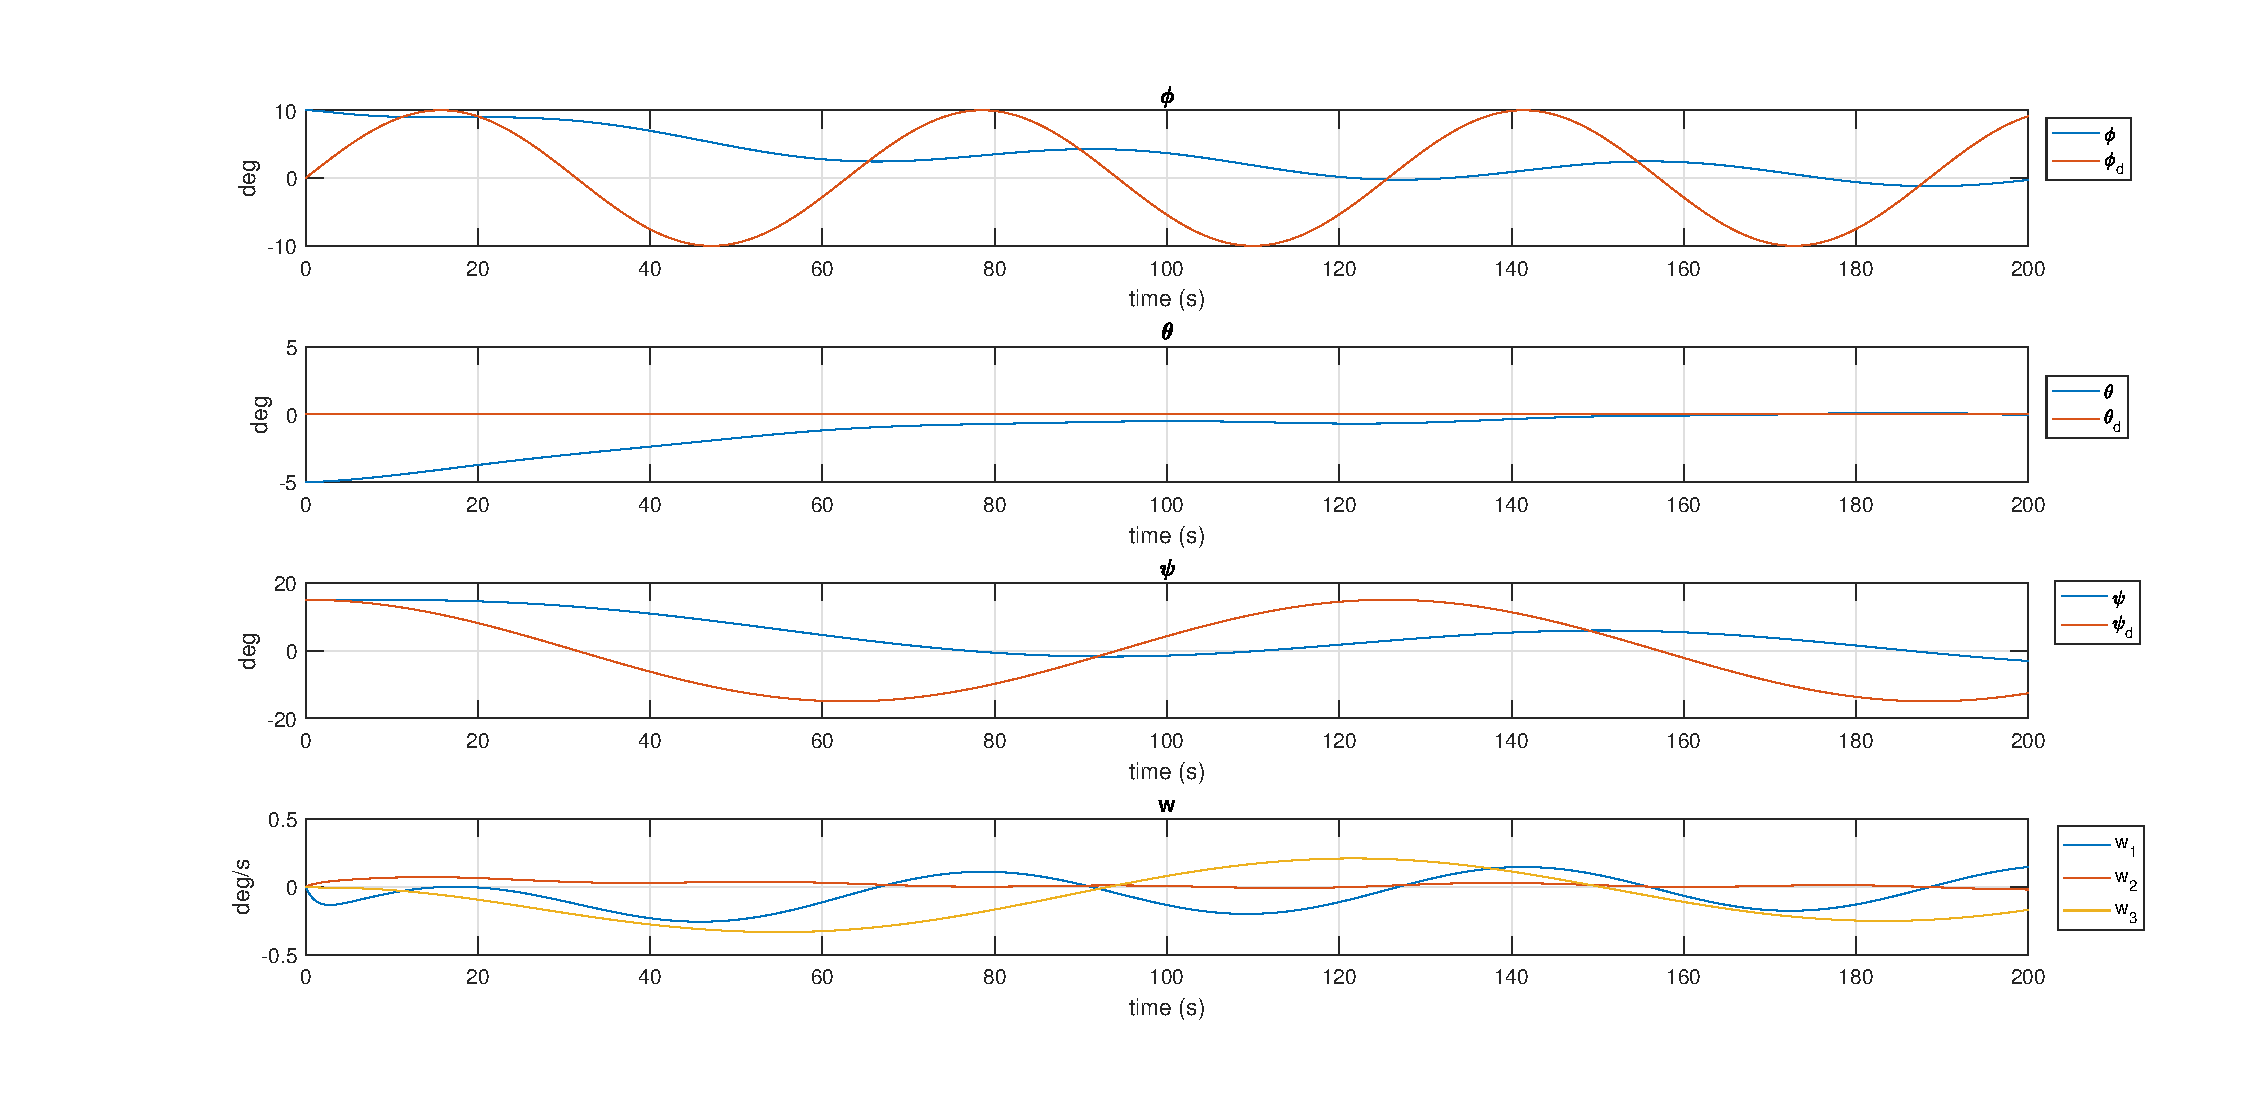
\includegraphics[width=1.00\textwidth]{figures/2_euler.eps}
	\caption{The resulting output euler angles with their corresponding desired values and the resulting output $\omega$ (denoted $\mathbf{w}$ in the plot) from the simulation in attitude2.}
\label{fig:sim_attitude2_euler}
\end{figure}

\begin{figure}
	\centering
	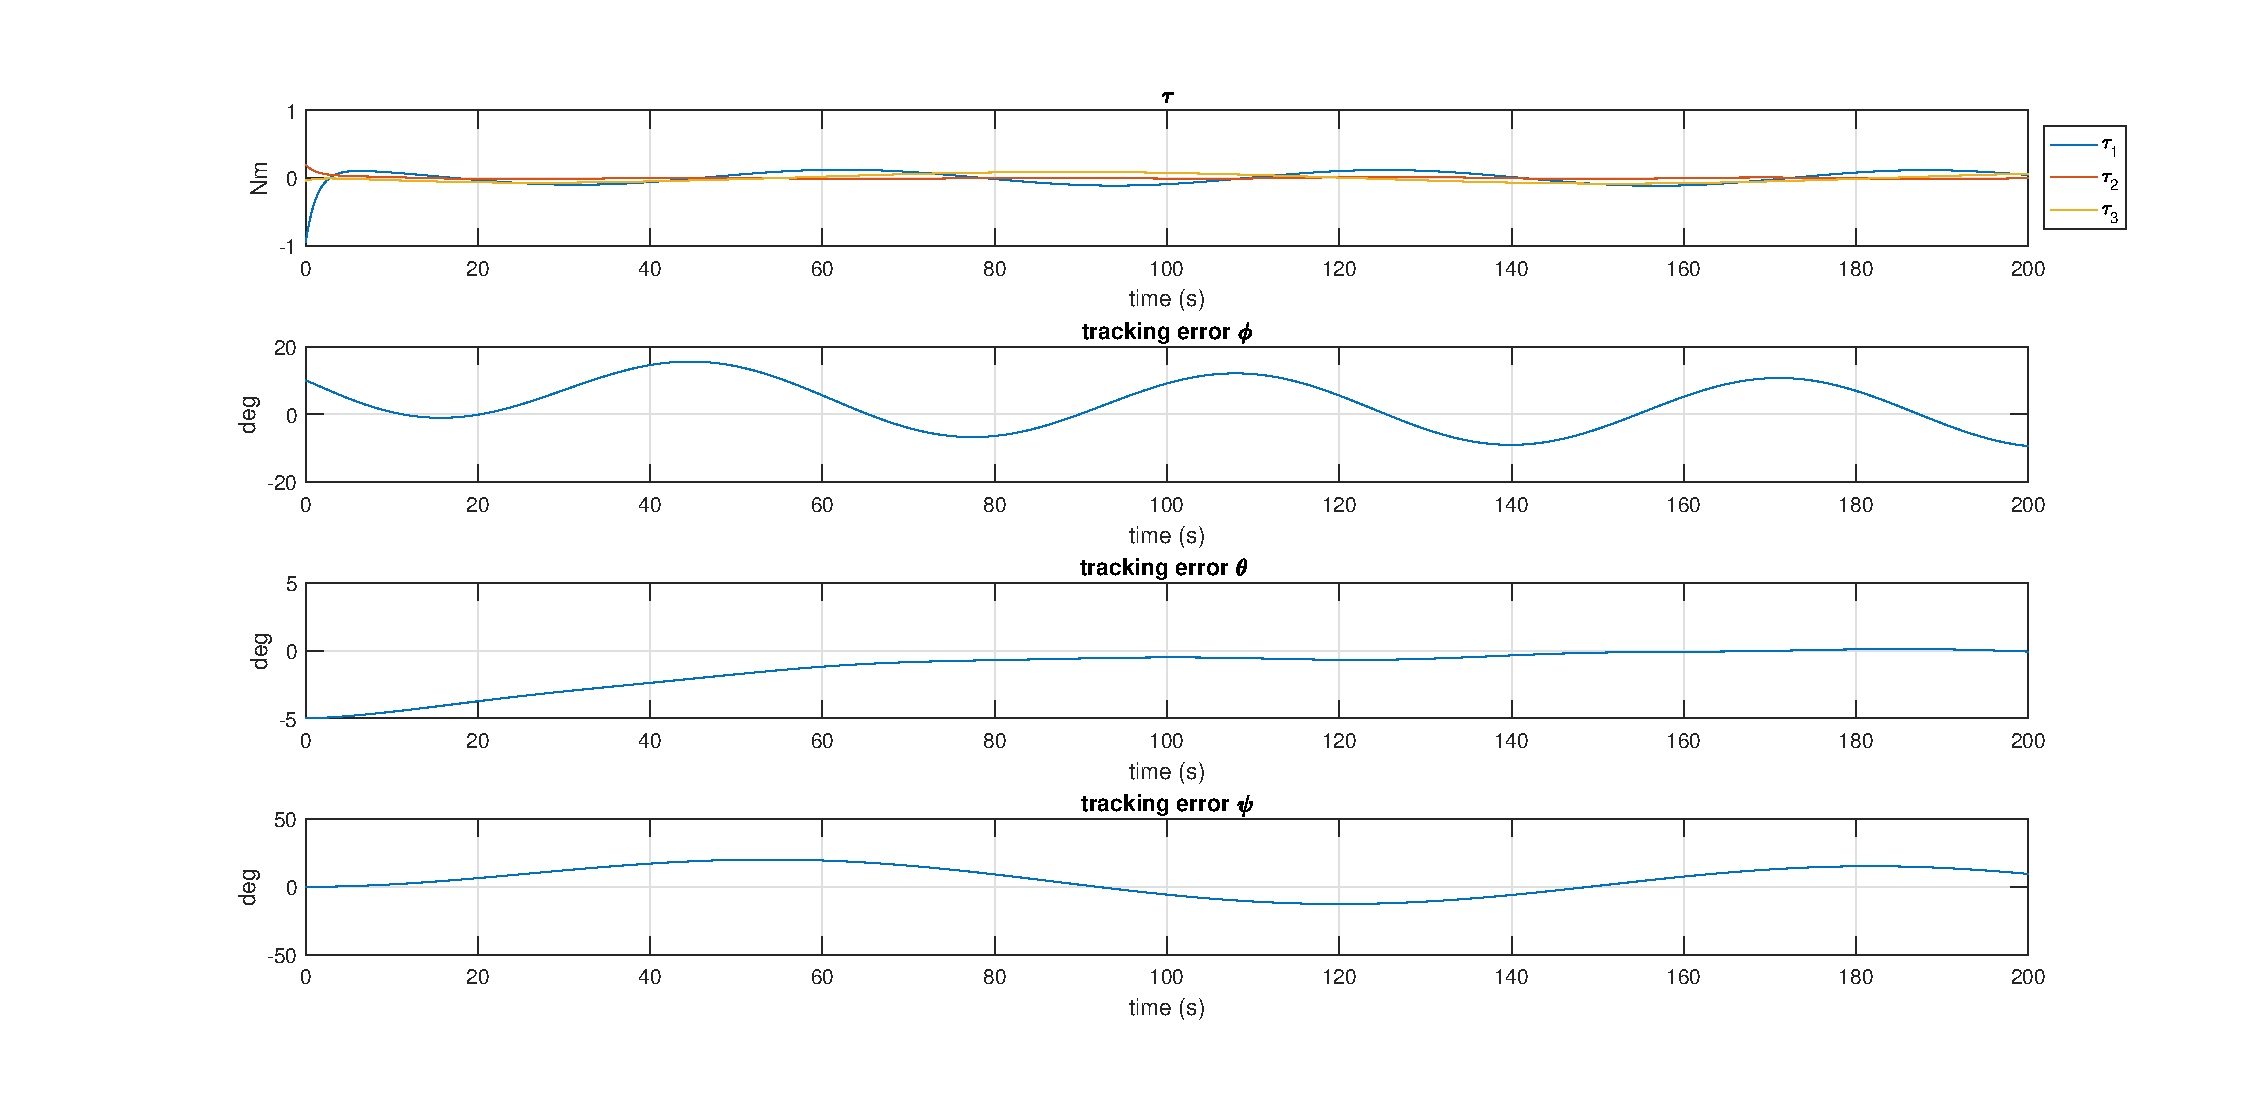
\includegraphics[width=1.00\textwidth]{figures/2_tau_track.eps}
	\caption{ $\tau$, and the tracking errors of the output euler angles from the simulation in attitude2.}
\label{fig:sim_attitude2_track}
\end{figure}

The Figures show that, with the exception of $\theta$, the angles of the satellite are following a sinusoidal pattern as per their desired values. However, they are not in sync with the desired signal and the amplitude is far too low compared to their intended forms, resulting in relatively large sinusoidal tracking errors as can be seen in \Cref{fig:sim_attitude2_track}. One reason for this misbehaviour is the fact that, even though the angles of the satellite is set to move in a specific way, the desired value of $\omega$ is still set to 0. This makes for a contradiction in the controller where neither part is able to do as they are told. The exception is $\theta$ and $\omega_1$ who are both set to 0.

It is also worth mentioning that the $\mathbf{K}$ matrix used for the controller was found using the linearized version of the system. This may also introduce errors.

\subsection*{Problem 1.6}

The attitude control law was modified to:
\begin{equation}
    \tau = -\mathbf{K}_d\tilde{\omega} -k_p\tilde{\epsilon}
    \label{eq:control_law_attitude3}
\end{equation}
\todo{Skal omega være i bold? Det er  ikke det i oppgaveteksten}

with $\tilde{\omega} = \omega - \omega_d$. Differentiating the desired attitude, $\Theta_d$, from the previous problem and calculating $\omega_d$ as

\begin{equation}
    \omega_d = \mathbf{T}_{\Theta_d}^{-1}(\Theta_d)\dot{\Theta_d}
    \label{eq:omega_d}
\end{equation}

We used the MATLAB function \texttt{eulerang()} to get the $\mathbf{T}_{\Theta_d}$ and set $k_p$ and $k_d$ to 10 and 300 respectively as before and used the $\omega_d$ calculated from \eqref{eq:omega_d} in the new simulation {\color{blue} attitude3.m}.

\subsubsection*{Simulation results}

We can see from \Cref{fig:sim_attitude3_euler} and \Cref{fig:sim_attitude3_omega} that the satellite is now able to follow the given reference signal for both angles and angle velocities. From \Cref{fig:sim_attitude3_track} we can see that though there still is an error in the $\phi$ and $\psi$ they are much smaller than previously. Now that $\omega$ and $\epsilon$ have corresponding desired values, they can both be satisfied by the same actions. The cooperation between the two parts of the state, which are in themselves related, is key to making a good controller. The linearization error discussed in the previous problem may still endure and the controller is not exactly the fastest in the galaxy, but all in all the satellite control is much better than before.

\begin{figure}
	\centering
	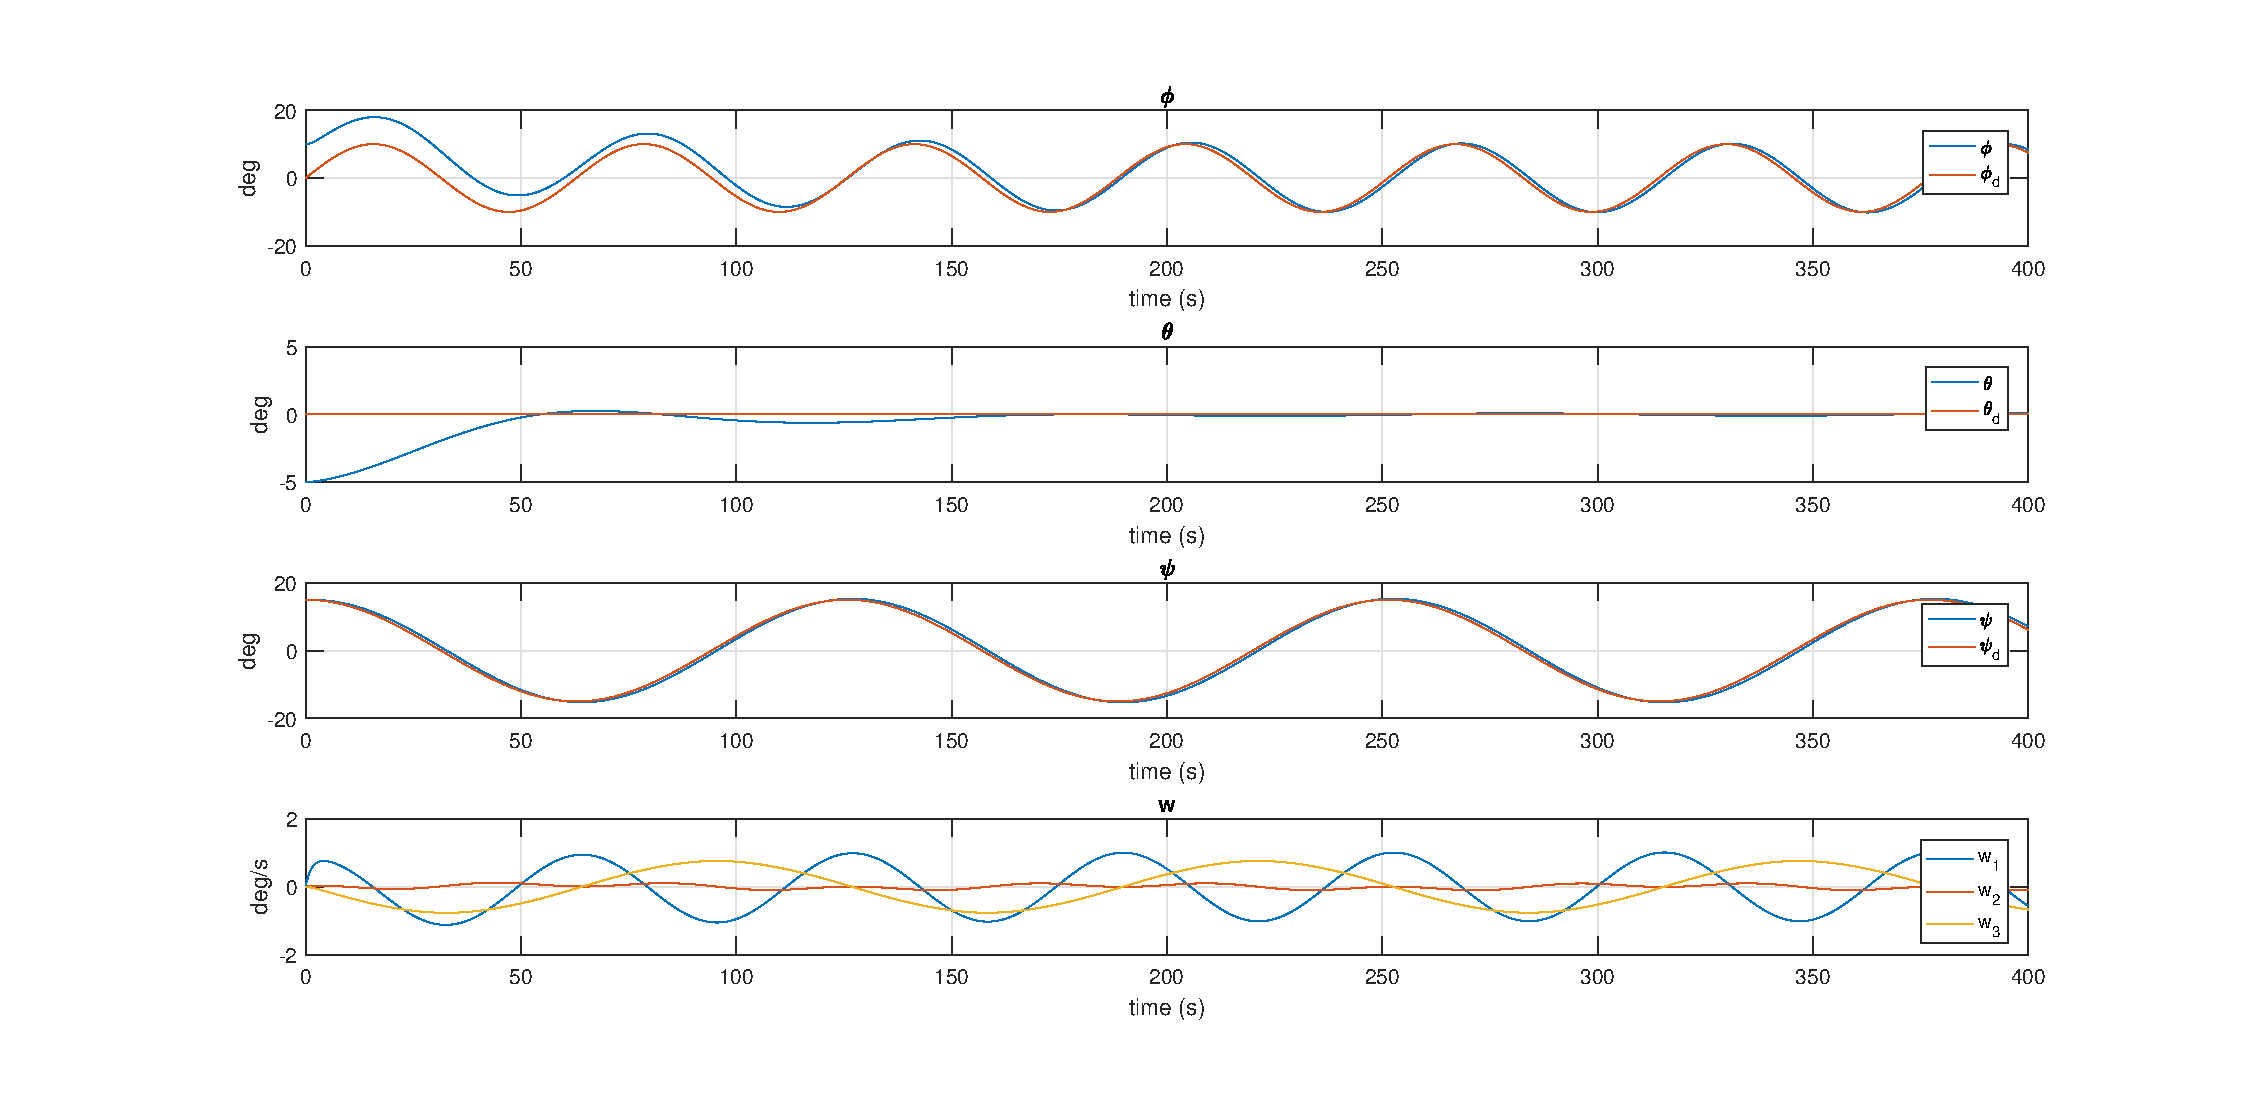
\includegraphics[width=1.00\textwidth]{figures/3_euler.eps}
	\caption{The resulting output euler angles with their corresponding desired values from the simulation in attitude3.}
\label{fig:sim_attitude3_euler}
\end{figure}

\begin{figure}
	\centering
	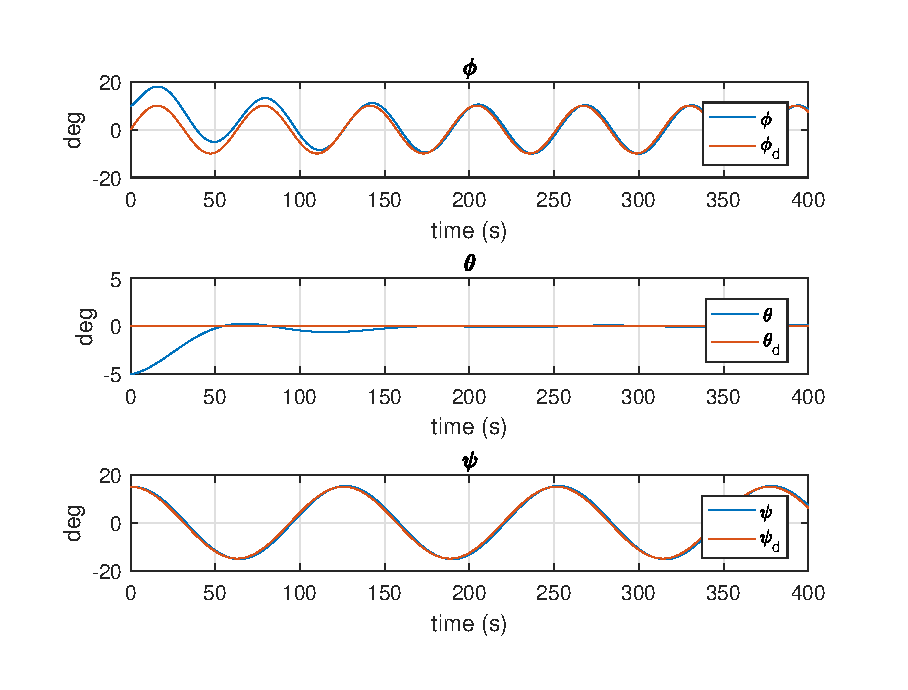
\includegraphics[width=1.00\textwidth]{figures/3_omega.eps}
	\caption{The resulting output $\omega$ (denoted $\mathbf{w}$ in the plots) and the corresponding desired values from the simulation in attitude3.}
\label{fig:sim_attitude3_omega}
\end{figure}

\begin{figure}
	\centering
	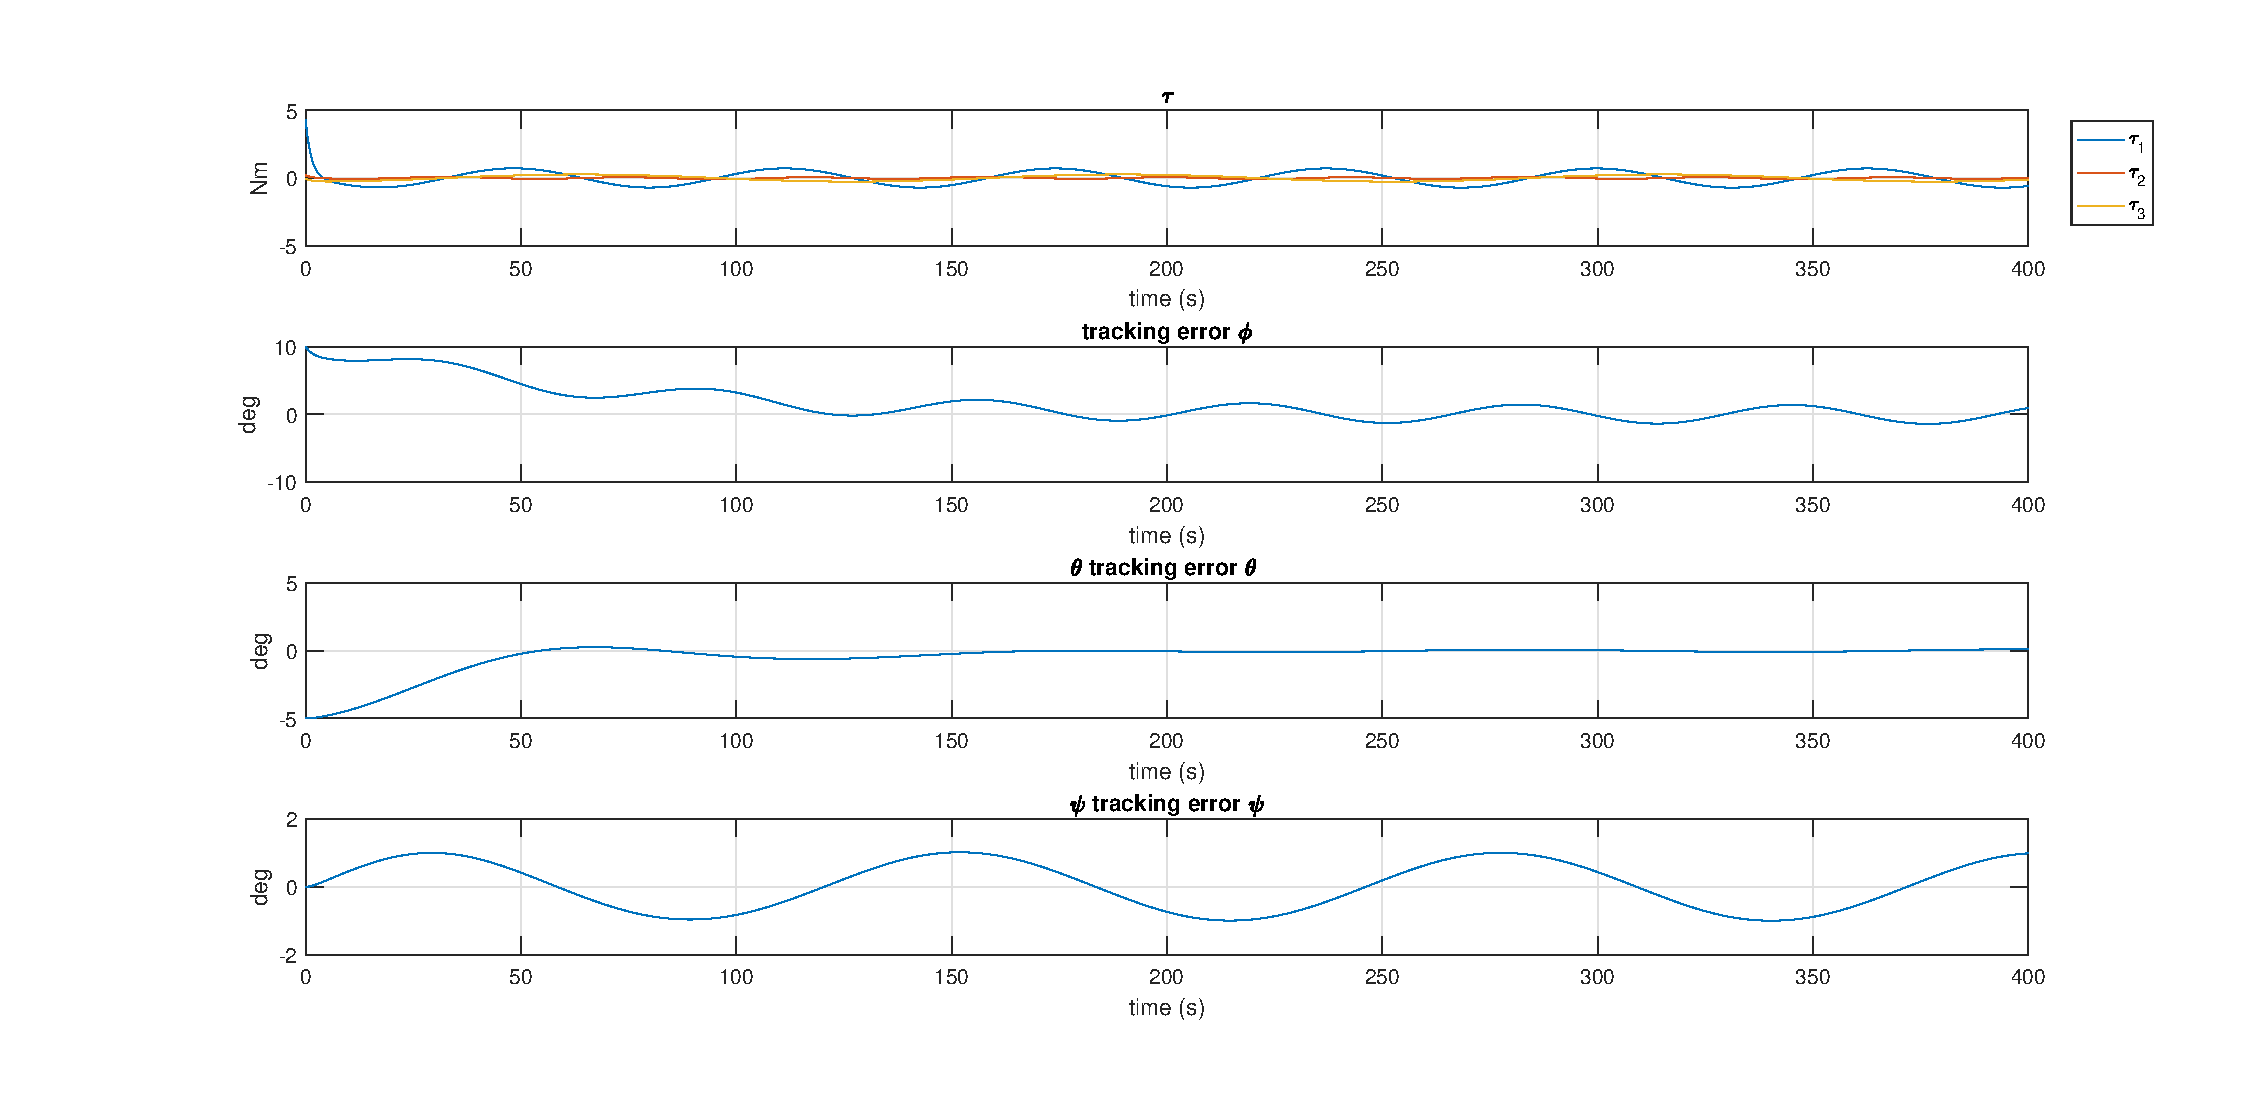
\includegraphics[width=1.00\textwidth]{figures/3_tau_track.eps}
	\caption{ $\tau$, and the tracking errors of the output euler angles from the simulation in attitude3.}
\label{fig:sim_attitude3_track}
\end{figure}

\subsection*{Problem 1.7}
Assuming $\omega_d = 0$ and $\epsilon_d$ and $\eta_d$ constants and the control law given by \eqref{eq:control_law_attitude2}, the Lyapunov function 
 \begin{equation}
	 V = \frac{1}{2} \tilde{\boldsymbol{\omega}}^{\top} \mathbf{I}_{CG}\tilde{\boldsymbol{\omega}} + 2 k_p (1-\tilde{\eta})
 \end{equation}
 
is positive and radially unbounded. 

The reason for its positivity is that $\mathbf{I}_{CG}$ being an identity matrix with a positive number, $mr^2$, on its diagonal, is positive definite. So the first part of V is positive (labeling 0 as a positive number). The second part, consisting of $2 k_p (1-\tilde{\eta})$, may only be negative if $\tilde{\eta} > 1$. This will never happen however, as $\tilde{\eta}$ is part of the unit quaternion $\tilde{q}$ making $|\tilde{\eta}| \leq 1$. Thus the second part of V will also be positive. The Lyapunov function is usually thought of as a representation of the energy in the system so the fact that it is never negative makes sense. 

The function is radially unbounded because as $\tilde{\omega}\rightarrow \infty$ the first part of V does the same, $\frac{1}{2} \tilde{\boldsymbol{\omega}}^{\top} \mathbf{I}_{CG}\tilde{\boldsymbol{\omega}} \rightarrow \infty$. We already established that the second part of V, $2 k_p (1-\tilde{\eta})$ is positive, meaning that V as a whole is unbounded.

To calculate $\dot{V}$ $\tilde{\omega} = \omega - \omega_d = \omega$ was substituded into V before differentiating:

\begin{equation}
    \dot{V} = \omega^\top\mathbf{I}_{CG}\dot{\omega} + k_p\tilde{\epsilon}^\top\omega 
\end{equation}

Then, using \eqref{eq:EOM_omega_dot}, $\mathbf{I}_{CG}\dot{\omega}$ was substituted:

\begin{equation}
    \dot{V} = \omega^\top(\tau - \mathbf{S}(\mathbf{I}_{CG})\omega) + k_p\tilde{\epsilon}^\top\omega 
\end{equation}

Knowing $\omega\mathbf{S}(\mathbf{I}_{CG})\omega = 0$ and substituting $\tau$ from the control law in \eqref{eq:control_law_attitude2} we are left with

\begin{equation}
    \dot{V} = \omega^\top( k_d \omega - k_p\tilde{\epsilon}) + k_p\tilde{\epsilon}^\top\omega = -k_d\omega^\top\omega
\end{equation}

Barbalat's lemma tells us that our $\omega$ will converge to zero if three conditions are satisfied: 

\begin{itemize}
    \item $V \geq 0$
    \item $\dot{V} \leq 0$
    \item $\dot{V}$ is uniformly continuous
\end{itemize}

We already proved the first one when we proved V is positive. For the second condition we can easily see that $\dot{V}$ as a negative quadratic function, due to $\omega^\top\omega \geq 0$ and $k_d \geq 0$ a constant, must be $\leq 0$.

To prove $\dot{V}$ is uniformally continuous, we can take a look at $\ddot{V} = -2k_d\omega^\top\dot{\omega}$ and prove it to be bounded. We can assume the $\omega$, and thereby V, does not begin at $\infty$ and we know $\dot{V}$ is negative, meaning V is always sinking. However V will always be positive, meaning it must stop at 0. Thus $\omega$ will never increase beyond it's initial value. Knowing we are in physical system, it is reasonable to assume $\omega$ is continuous, thus $\dot{\omega}$ cannot go towards $\infty$. With neither $\omega \rightarrow \pm\infty$ nor $\dot{\omega} \pm\rightarrow \infty$, $\ddot{V} = -2k_d\omega^\top\dot{\omega}$ is bounded. Meaning $\dot{V}$ is uniformly continuous and Barbalat is satisfied. $\omega$ will converge to zero. \todo{Spør om dette}

According to the corriculum book\cite{Fossen2011}, Barbalat's lemma only guarantees global convergence, meaning our convergence to the equilibrium point is indeed global.

\subsubsection*{Asymptotic stability}

We have a non-autonomous system so to check stability we may take a look at LaSalle-Yoshizawa's teorem. It states that

\begin{itemize}
    \item $V > 0$ and  $V(0) = 0$
    \item $\dot{V} \leq 0$
    \item V is radially unbounded
\end{itemize}

We have already proved the last two

\todo{What about W?}

\subsection*{Problem 1.8}
...

% Note that \mathbf can be used for bold letters in math mode (within equations and dollar signs). \boldsymbol can be used to get bold greek letters.  


\section*{Problem 2 - Underwater Vehicles}
\addcontentsline{toc}{section}{Problem 2 - Underwater Vehicles }
For part 2 of this assignment the focus shifted from the satellite in space to an Underwater Vehicle. For the entirety of this part the vehicle moves at a constant depth $z=10m$ at a speed of $U=1.5m/s$ and a pitch angle of $\theta = 2.0^\circ$ and a roll angle of $\phi = 0^\circ$. While moving on a straight line the course angel was given $\chi = 30^\circ$.
\subsection*{Problem 2.1}
\addcontentsline{toc}{subsection}{Problem 2.1}
The crab angle is given by the equation:
\begin{equation}
    \beta = \chi - \psi
\end{equation}

Assuming there no currents and $\beta = 0$, the resulting heading is $\psi = \chi = 30^\circ$.

Another formulation for the crab angle is

\begin{equation}
    \beta = sin^{-1}(\frac{v}{U})
\end{equation}

Using this, the known value of U and the fact that $\beta$ is still assumed to be zero we can calculate v, resulting in $v=0$

When it comes to the rest of the entries of the velocity vector one could choose to calculate them using basic trigonometry, using the angle between the velocity vector and the x-axis of the body frame to calculate its u and w parts. Alternatively one could choose to use the equations for rotating from flow coordinates to body coordinates from the course book \cite{Fossen2011}. For both methods $\beta$ is noted to be zero and they both means recognizing the remai

\subsection*{Problem 2.2}
\addcontentsline{toc}{subsection}{Problem 2.2}
Answer Problem 2.2 here. The body-fixed velocities can be written as
\begin{equation}
\label{eq:velocity}
	\begin{bmatrix}
		u \\
		v \\
		w
	\end{bmatrix}
	= 
	\begin{bmatrix}
		U \cos( \omega t)\\
		U \sin(\omega t)\\
		0	
	\end{bmatrix}
\end{equation}

\subsection*{Problem 2.3}
\addcontentsline{toc}{subsection}{Problem 2.3}

Answer Problem 2.3 here.

EQUATIONS ELLA NEED ;)
\begin{equation}
    \begin{aligned}
    \mathbf{v}_c^n 
    =
    \begin{bmatrix}
    U_c \cos(\alpha_c) \cos(\beta_c) \\
    U_c \sin(\beta_c) \\
    U_c \sin(\alpha_c) \cos(\beta_c)\\
    \end{bmatrix}
    \label{eq:v_n_c}
    \end{aligned}
\end{equation}

\begin{equation}
    \boldsymbol{v}_r = \boldsymbol{v} - \boldsymbol{v}_c
    \label{eq_v_r}
\end{equation}

% Ella-Lovise  is writing

\subsection*{Problem 2.4}
\addcontentsline{toc}{subsection}{Problem 2.4}

\subsubsection*{Calculate sideslip angle}
\addcontentsline{toc}{subsubsection}{Calculate sideslip angle}

The sideslip angle is the angle from $x_b$ axis of {b} to the velocity vector of the vehicle, with positive rotation around the $z_b$ axis of {b} as given by the right-hand screw convention. The formula for sideslip is therefore:

\begin{equation}
    \boldsymbol{\beta}_r = \arcsin( v^b_r/U^b_r)
    \label{eq:beta_r}
\end{equation}

defined by the relative velocity $v_r$, from $\mathbf{V_r} = [u_r,v_r,w_r]^\top$, and relative speed $U_r$. The relative velocity in body frame in this assignment is defined by equation \eqref{eq:v_r}.The crab angle is defined in body, according to Fossen. In this assignment the relative velocity was defined to $\mathbf{v}^b_{b/n} = [1.5, 0,0]$, from problem 2.1. In problem 2.1 there was no current, and following the convention from problem 2.2, the velocity on a straight line relative to the ocean is given as $\mathbf{v}^b_{b/c} = [1.5, 0,0]$. \todo{åpen for omformuleirnger her ! } 

The sideslip angle was calculated using equation \eqref{eq:beta_r}, giving $0 ^\circ$. This result is as expected, since the relative velocity consists of $v=0$, and  $\mathbf{v}^b_{b/c} = [1.5, 0,0]$.  Because sideslip angle is defined by the relative velocities, and the vehicle tries to stick to a straight line, in reality the current will inflict a force upon the vehicle in a manner that will change the slope of the straight line, since the current is constant .  a   The result of the current carrying the vehicle will be noticeable on the crab angle, as discussed in later sections. 

\subsubsection*{Simulation of translational motion of the vehicle }
\addcontentsline{toc}{subsubsection}{Simulation of translational motion of the vehicle}

The simulation of the translational motion was performed using \texttt{MATLAB}. The initial conditions were $\phi = 0^\circ$, $\theta = 0^\circ$ and $\psi = 30^circ$ and start position at $\mathbf{0}$. With no current, $\mathbf{v}^b_{b/c} = \mathbf{v}^b_{b/n}$. To simulate the translational motion without current, the velocity of the vehicle relative to the ned was first calculated:
\begin{equation}
    \mathbf{v}^n_{b/n} = \mathbf{R}^n_b \mathbf{v}^b_{b/n} = \mathbf{R}^n_b [U \cos(\omega t), U \sin(\omega t), 0]^\top
    \label{eq:v_n_b_c}
\end{equation}


The position of the vehicle was found using Euler integration, meaning the position of vehicle is $\mathbf{p}\text{(i+1)}^n_{b} = \mathbf{p}(i)^n_{b} + \mathbf{v}(i)^n_{b/n}*h $, with timestep $h = 0.1$ and i equal the number of the iteration.
 
The  plotting of the translational motion with current, was also chosen to be in NED reference frame with the position relative to the NED, meaning $\mathbf{p}^n_{b}$. The first step was to calculate the velocity of the vehicle $\mathbf{v}^n_{b/c}$, as done in \eqref{eq:v_n_b_c}. Furthermore the velocity of the current relative to NED expressed in NED reference frame, $\mathbf{v}^n_{c/n}$ ,was calculated from equation \eqref{eq:v_n_c}. The expression for the velocity of the vehicle relative to NED  in NED reference frame is:


\begin{equation}
    \mathbf{v}^n_{b/n} = \mathbf{v}^n_{b/c} + \mathbf{v}^n_{c/n} = \mathbf{R}^n_b \mathbf{v}^b_{b/c} + \mathbf{v}^{n}_{c/n} 
    \label{eq:v_b_r}
\end{equation}

The expression for the position of the vehicle relative to NED reference frame is found by Euler integration, meaning $\mathbf{p}\text{(i+1)}^n_{b} = \mathbf{p}(i)^n_{b} + \mathbf{v}(i)^n_{b/n}*h $. The method used is the same as for the simulation without current.


The crab, course  and sideslip angle was calculated using respectively equation \eqref{eq:beta_2}, \eqref{eq:chi} and \eqref{eq:beta_r}, respectively. With $\mathbf{v}_r = \mathbf{v}^n_{b/c}$.  Because the arcsin command in \texttt{MATLAB}, \texttt{asin} only provides the angle between $-\frac{\pi}{2}$ and $\frac{\pi}{2}$,the crab angle and sideslip is approximated using atain2. This approximation is based on the assumption $w= 0$ and gives:

\begin{equation}
\begin{aligned}
	& \beta = atan2(v^b_{b/n}, u^b_{b/n} ) \\
	& \beta_r = atan2(v^b_{b/c}, u^b_{b/c} )  \\
	\label{eq:crab_slip_approx}
\end{aligned}
\end{equation}

\subsubsection*{Result after simulation}
\addcontentsline{toc}{subsubsection}{Result after simulation}

In \ref{fig:4_pos} the position of the vehicle relative to the NED is plotted using reference frame NED. Without current the vehicle makes a perfect circle with radius 100 m, as required and expected. With current the vehicle tries to make a perfect circle, but the current carries the vehicle in north-east direction, making the path to the vehicle relative to the ocean look like a spiral.

\begin{figure}[!ht] 
	\centering
	\begin{subfigure}[b]{0.45\textwidth}
		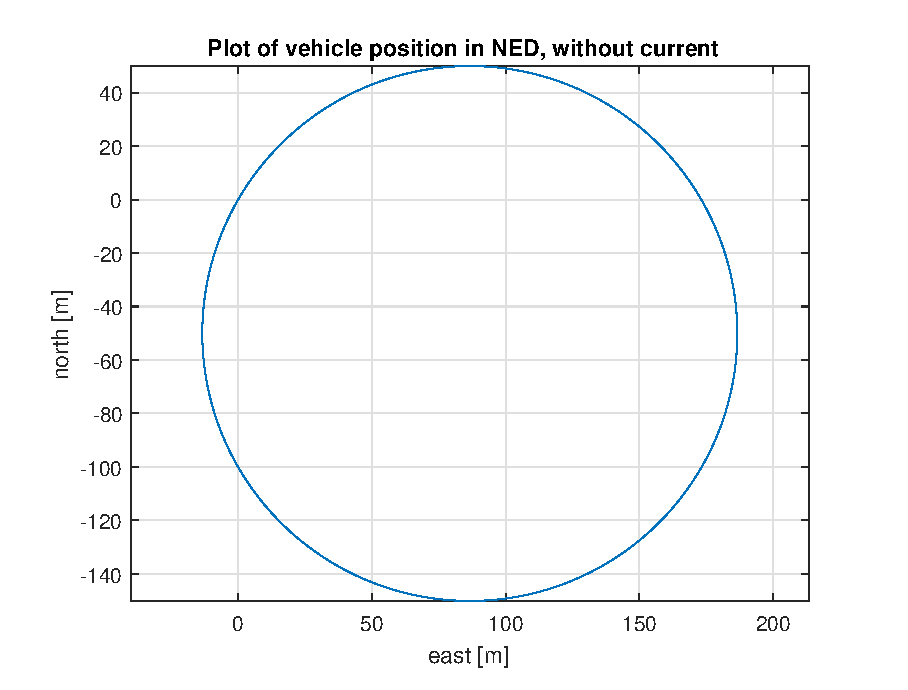
\includegraphics[width=\textwidth]{figures/4_pos.eps}
		\caption{Without current}
		%\label{fig:4_pos}
	\end{subfigure}
	~ %add desired spacing between images, e. g. ~, \quad, \qquad, \hfill etc. 
	%(or a blank line to force the subfigure onto a new line)
	\begin{subfigure}[b]{0.45\textwidth}
		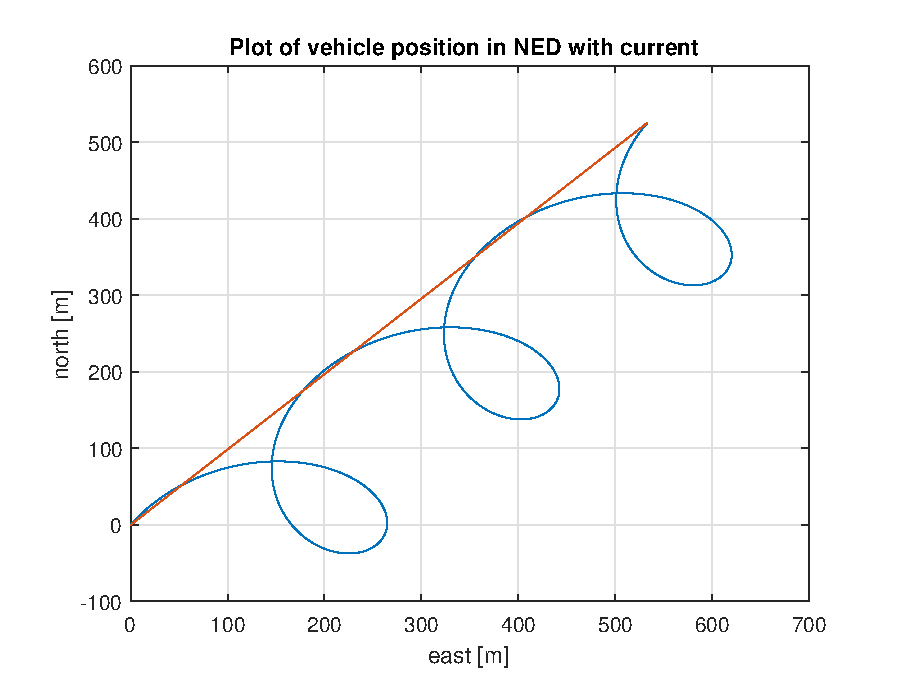
\includegraphics[width=\textwidth]{figures/4_pos_current}
		\caption{With current. The red line marks the flow of the current, the blue the position of the vehicle}
		\label{fig:4_pos_current}
	\end{subfigure}
	\caption{The position of the vehicle in reference frame NED}
	\label{fig:4_pos}
\end{figure}

The relative velocities will be the same with and without current. The vehicles velocity in body frame relative to current is defined ad $\mathbf{v}^b_{b/c} = [U \cos(\omega  *t), U \sin(\omega*t) , 0]$ and hence will not depend on current, $\omega$ is constant. This is shown in figure \figref{fig:4_vel}, which demonstrates the velocity of vehicle relative to the ocean current in NED reference frame. The plot in \figref{fig:4_vel} a) shows constant speed, since $\mathbf{v}^b_{b/c}$ consists of a cosine and sinusoidal  depending on both frequency and time. 

A plot of velocity  $\mathbf{v}^n_{b/n}$ affected by current is shown in figure \figref{fig:4_vel} b) . Since there is current   looking at the velocity of the body relative to NED, both the speed and velocity is  affected by the current. Because the relative velocity is $\mathbf{v}_r = v + v_c$, and $\mathbf{v}_c != \mathbf{0}$, the speed is not constant, but varies sinusoidal. The same goes for the velocity $\mathbf{v}^n_{b/n}$, affected by the constant current velocities. The reason for  $\mathbf{v}^n_{b/n}$ being periodically is that both the current and the relative velocity of the vehicle is periodic.

\begin{figure}[!ht]
	\centering
	\begin{subfigure}[b]{0.45\textwidth}
		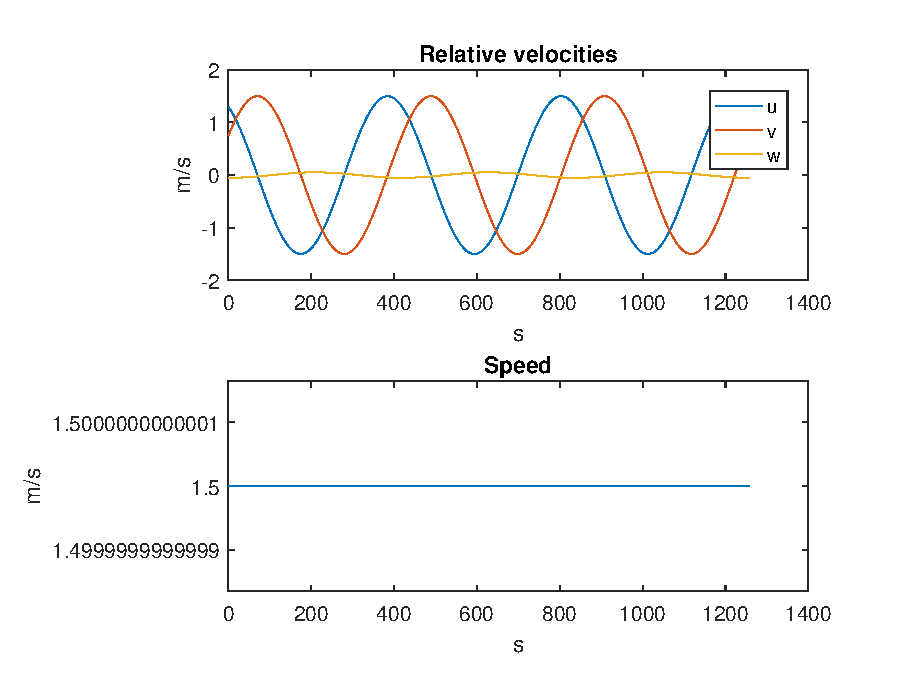
\includegraphics[width=\textwidth]{figures/4_vel}
		\caption{Without current}
		%\label{fig:4_vel}
	\end{subfigure}
	~ %add desired spacing between images, e. g. ~, \quad, \qquad, \hfill etc. 
	%(or a blank line to force the subfigure onto a new line)
	\begin{subfigure}[b]{0.45\textwidth}
		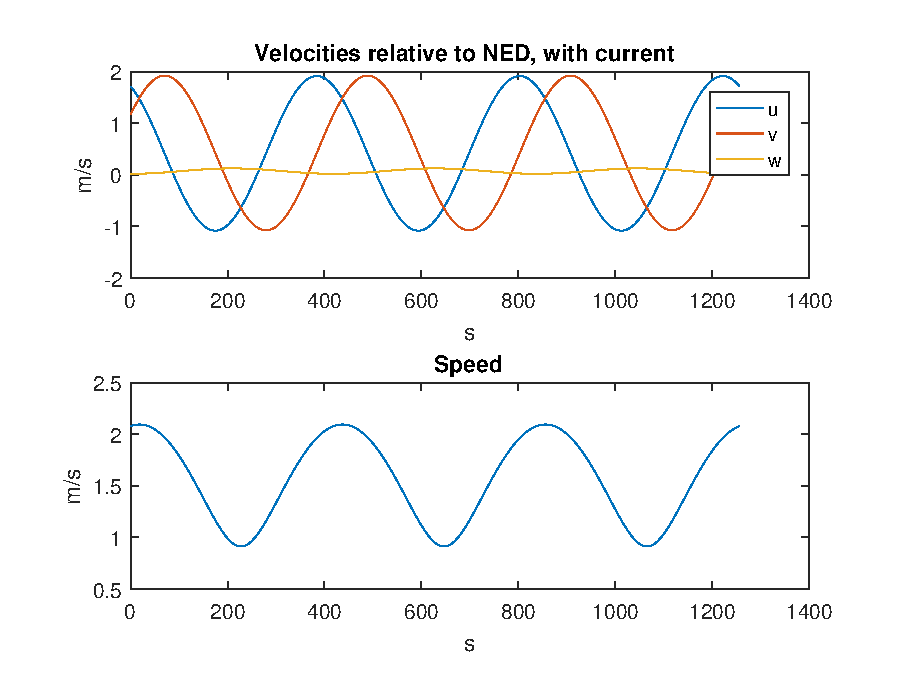
\includegraphics[width=\textwidth]{figures/4_vel_ned_with_cur}
		\caption{With current}
		%\label{fig:4_vel_ned_with_cur}
	\end{subfigure}
	\caption{The relative velocity and speed of the vehicle, defined equation \eqref{eq:v_n_r} in reference frame NED}
	\label{fig:4_vel}
\end{figure}


The plots of crab, sideslip and course angle is in figure \ref{fig:4_crab}. Crab, sideslip and course angle goes from $0-360^\circ$, all plots in this report restricted angles to stay within 0-360 degrees. It is reasonable that  the anlges goes from $0-360^\circ$ since the vehicle is driving in a circle with the bow  in the same direction. In the plot without current $\mathbf{v}^b_{b/c} = \mathbf{v}^b_{b/n} $, this means $\beta_r = \beta$, which is also clear from the plot. In the plot with current the sideslip angle $\beta_r$ is the same as in plot without current. The crab angle and course angle which depends upon the velocity of the current is therefore different in the plot with current. Since there is current, the relationship between $u^b$ and $v^b$ varies periodically, meaning the crab and course angle varies periodically. The reason for this is that the course angle  is linearly dependent upon crab angle and yaw. 

\begin{figure}[!ht]
	\centering
	\begin{subfigure}[b]{0.45\textwidth}
		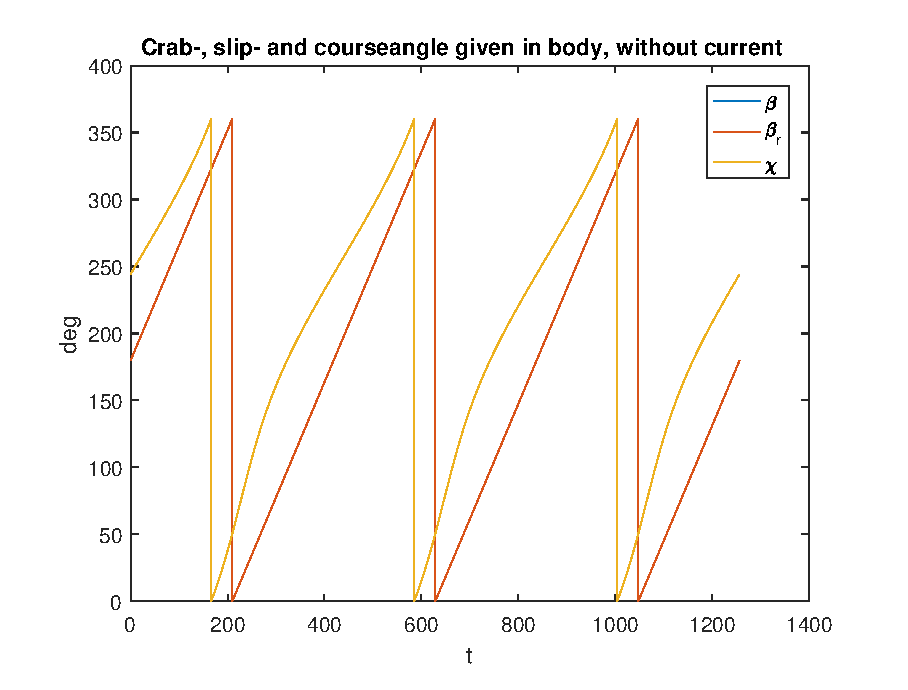
\includegraphics[width=\textwidth]{figures/4_crab_slip_course}
		\caption{Without current}
		%\label{fig:4_vel}
	\end{subfigure}
	~ %add desired spacing between images, e. g. ~, \quad, \qquad, \hfill etc. 
	%(or a blank line to force the subfigure onto a new line)
	\begin{subfigure}[b]{0.45\textwidth}
		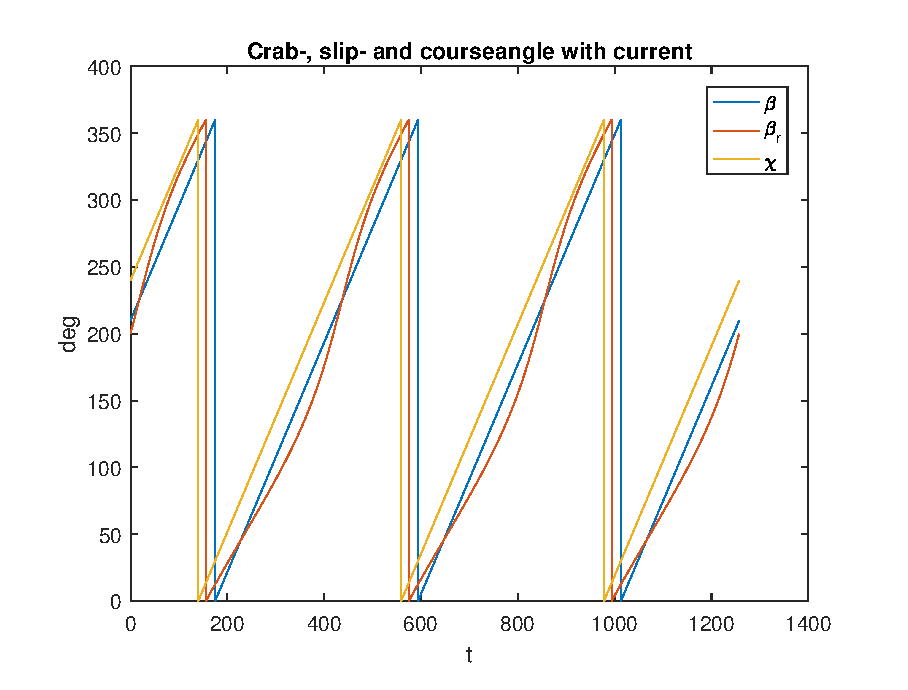
\includegraphics[width=\textwidth]{figures/4_crab_slip_course_current}
		\caption{With current}
		%\label{fig:4_vel_current}
	\end{subfigure}
	\label{fig:4_crab}
	\caption{The crab-, course and sidslip angles in reference frame NED}
\end{figure}

\subsection*{Problem 2.5}
\addcontentsline{toc}{subsection}{Problem 2.5}

The vehicle's turning rates are now assumed to be modeled by the Nomoto model and are:
\begin{equation}
	\frac{r}{\delta} (s) = \frac{K}{Ts+1}
\end{equation}

with $\delta$ equal the rudder angle, $K =0.1 s^{-1}$ and $T = 50s$.

The pitch and roll motions are given as
\begin{equation}
\begin{aligned}
	&\dot{p} + 2\zeta_p\omega_p p + \omega_p^2 \phi = 0\\
	&\dot{q} + 2\zeta_q\omega_q q + \omega_q^2 \theta = 0
	\label{eq:p_q_dot}
\end{aligned}
\end{equation}
with damping factors and natural frequencies as $\zeta_p = 0.1 $, $\zeta_q = 0.2 $, $\omega_p = 0.1 $ and $\omega_q = 0.05 $. 

\subsubsection*{Calculations of steady state}
\addcontentsline{toc}{subsubsection}{Calculations of steady state}

The steady state angular velocities $p_s$, $q_s$ and $r_s$ during turning for a constant rudder angle $\delta$ may be found by setting $\dot{p}= \dot{q} = \dot{r} = 0$. The equation for $\dot{r}$ may be found by applying the inverse Laplace using the Nomoto equation. In \cite{Fossen2011} the time representation of the first order Nomotos model, equation (7.52) in \cite{Fossen2011} is estimated as 

\begin{equation}
    T\ddot{\psi} + \dot{\psi} = K \delta
    \label{eq:nomo_first_order_time}
\end{equation}

In this problem $\theta = 2.0 ^\circ$ and $\phi = 0.0 ^\circ$, giving $\dot{\psi}$ as approximately $r$. Using \eqref{eq:nomo_first_order_time} the  first order Nomoto-model time representation is given as:

\begin{equation}
    \dot{r} = - \frac{r}{T} +  \frac{K}{T} \delta
    \label{eq:r_time}
\end{equation}

Using \eqref{eq:r_time} and \eqref{eq:p_q_dot} and setting $\dot{p} =\dot{q} = \dot{r}$ this gives the following expression for the steady state of the angular  velocities:

\begin{equation}
\begin{aligned}
	& p_s = \frac{\omega_p^2 \phi}{ 2\zeta_p\omega_p} = \frac{1}{2} \phi \\
	& q_s = \frac{\omega_q^2 \theta}{2\zeta_q\omega_q} = \frac{1}{8} \phi \\
	& r_s = K \delta
	\label{eq:p_q_dot}
\end{aligned}
\end{equation}

This means the steady state angular velocities $p_s = \frac{1}{2} \phi ^\circ s^{-1}$, $q_s = \frac{1}{9} \theta ^\circ s^{-1}$, $r_s = 0.1 \delta ^\circ s^{-1}$. 

\subsection*{Problem 2.6}
\addcontentsline{toc}{subsection}{Problem 2.6}

In this problem the model of the vehicle is implemented by varying $\boldsymbol{\omega}^b_{b/n}$, described in equation \eqref{eq:r_time} and \eqref{eq:p_q_dot}. The system have the initial positions $\boldsymbol{\Theta} = [-1.0^\circ, 2,0^\circ, 0.0^\circ]^\top$ and $\boldsymbol{\omega}^b_{b/n} = [0,0,0]^\top s^{-1}$ . The start position is $\mathbf{p}^n_{b} = [0,0,0]^\top m$. The vehicle is still exposed to the current described in equation \eqref{eq:v_n_c}  and the rudder changes after 700 seconds from $\delta = 5^\circ$ to $\delta = 10^\circ$.

Since the current is constant in NED reference frame, the rotation of $\omega^n_{c/b} $ is zero, implying $\boldsymbol{\omega}^b_{c/b} = 0$. This means $ \boldsymbol{\omega}^b_{b/n} = \boldsymbol{\omega}^b_{b/c} + \boldsymbol{\omega}^b_{c/n}  = \boldsymbol{\omega}^b_{b/c} $. \todo{Should i be more spesific, or more wage ? What do you think Alexandra ? Seems plausible, but I'm no expert at this}

\subsection*{Simulation}
\addcontentsline{toc}{subsubsection}{Simulation}

The system is simulated in the file {\color{blue} attitude4.m}. The files start by initializing all the relevant variables. In the simulation the time step is $h = 0.1$ .

Because of varying $\boldsymbol{\omega}^b_{b/n}$, the Euler angles will change during the simulation. Consequently, the first thing to do for each iteration is to calculate the new rotation matrix $\mathbf{R}^n_b$, dependent on the current Euler angles. To find $ \dot{\boldsymbol{\Theta}}$ equation (2.40) in \cite{Fossen2011} was used. Equation (2.40) states:

\begin{equation}
    \begin{aligned}
    \begin{bmatrix}
    \dot{\mathbf{p}}^n_{b/n} \\
    \dot{\boldsymbol{\Theta}}_{nb} \\
    \end{bmatrix}
    =
    \begin{bmatrix}
    \mathbf{R}^n_{b}(\boldsymbol{\Theta}_{nb}) & \mathbf{0}_{3x3} \\
    \mathbf{0}_{3x3} & \mathbf{T}_\Theta (\boldsymbol{\Theta}_{nb})  \\
    \end{bmatrix}
    \begin{bmatrix}
    \mathbf{v}^b_{b/n} \\
    \mathbf{\omega}^b_{b/n} \\
    \end{bmatrix}
    \end{aligned}
    \label{eq:eta_dot_J_eta}
\end{equation}

To find $\mathbf{v}^n_{b/n}$ the $\mathbf{v}^b_{b/c} = [U \cos(rt), U \sin(r t),0]$ was calculated first using the turning rate $r$ described by the Nomoto equation \eqref{eq:r_time}. 

The velocity relative to NED is found using the constant current velocity relative to reference frame NED, , equation \eqref{eq:v_n_c}, and rotating the relative velocity of the boat to NED, giving the following equation:

\begin{equation}
    \mathbf{v}^n_{b/n} = \mathbf{R}^n_{b} \mathbf{v}^b_{b/c} + \mathbf{v}^n_{c/n}
\end{equation}

To find the position of the vehicle relative to NED in NED reference frame, again, Euler integration was used giving:
\begin{equation}
    \mathbf{p}^n_b(i+1) = \mathbf{p}^n_b(i) + \mathbf{v}^n_{b/n} * h
\end{equation}
with i equal to the iteration number.

Before the next iteration of the simulation-for-loop can start, the new $\boldsymbol{\omega}^b_{b/n}$ must be calculated. $\dot{p}$ and $\dot{q}$ is calculated using equation \eqref{eq:p_q_dot}, and $\dot{r}$ is calcualted using \eqref{eq:r_time}. Using Euler integration, the next $\boldsymbol{\omega}$ is found, giving:

\begin{equation}
\begin{aligned}
	& p\text{(i+1)} = p(i) + \dot{p} h \\
	& q\text{(i+1)} = q(i) + \dot{q} h \\
	& p \text{(i+1)} = p(i) + \dot{p} h
\end{aligned}
\end{equation}

The crab and sideslip angles are calculated using \eqref{eq:crab_slip_approx}, assuming  $w$ ,from $\mathbf{v} =[u,v,w]^\top$, is approximately zero. The course angle is calculated using \eqref{eq:chi}.


\subsubsection*{Discussion of result from simulation}
\addcontentsline{toc}{subsubsection}{Discussion of plots from simulation}

The plot of the Euler angles are presented in \figref{fig:2_6_ang}, and shows that $\theta$ and $\phi$ have small oscillations in the start, but with a steady state of approximately $\phi_s = 0$ and $\theta_s = 0$. The Euler angles depend on the angular velocities. In the plot of the angular velocities, \figref{fig:2_6_ang_vel}, there are noticeable oscillations to begin with. $p$ and $q$ oscillates in the transient before they
converges to 0, witch corresponds to mass-spring-damper systems. This is because of the initial values of the Euler angles are not zero.

There are dependencies between Euler angles and angular velocities through the transformation matrix, represented in equation \eqref{eq:eta_dot_J_eta}.  \todo{ Føler det er flere grunner....}. After a while $p$ and $r$ gets to steady state, which is approximately zero, as well as the Euler angles. In problem 2.5, we calculated an equation, equation \eqref{eq:omega_s} for the steady state values for $p$ and $q$.Using the steady state values for $\phi = 0$ and $\theta = 0$ gives $p_s = 0 deg/s$ and  $q_s = 0 deg/s$. This means $p$ and $q$ approaching calculated   steady state value.\todo{i am not sure...}  

The yaw is more or less growing linearly, going from $0-360 ^\circ$. This is consistent with $r = \dot{\psi}$, so that with constant rudder the yaw is linearly growing, as expected with a vehicle going in a circle, with a bow chaining directions. $r$ is expressed as an first order differential equation through the Nomoto model, and  figure \figref{fig:2_6_ang_vel} looks like the step response of a first order system. We get a step response because first $\delta = 5^\circ$ and after 700 seconds $\delta = 10^\circ$.  The change in the rudder is noticeable both in the plot of the yaw and in the plot of the r. In the plot of the yaw the slope is larger after 700 seconds, consistent with higher value of $r$. The transient of the $r$ is also noticeable on the yaw, with a slope of yaw not being linear. The angular velocity $r$ has two steady states, approximately  $0.5^\circ s^{-1}$  and $1.0^\circ s^{-1}$, this is consistent with the result from problem 2.5 with steady state value $r_s = K*\delta$, implying a steady state value of $r_s = 0.5^\circ s^{-1}$ and $1.0^\circ s^{-1}$. 

Looking at the steady state values of $\boldsymbol{\omega}^n_{b/n}$ there are approximately no angular velocities around $x_b$ and $y_b$, while around $z_b$ there is a constant angular velocity, meaning the vehicle will turn in a circle about $z_b$ as long as the rudder is nonzero. \todo{that do you think about the notaiton alexandra deg /sec osv. Den er grei :)}.

The change in pitch and roll angles as time passes makes sense from the perspective of the model. In our model of the vehicle, pitch , roll and yaw are as good as decoupled, especially in steady state. Looking at the plots of the Euler angles and the angular velocities, there are no connection between $\phi$ and $\theta$ and $r$, consistent with the equations of the system. In a realistic world, this is not true, and therefore roll and pitch would most likely be more affected by the change in yaw in the real world.\todo{anything to add ?}


\begin{figure}[!ht]
	\centering
	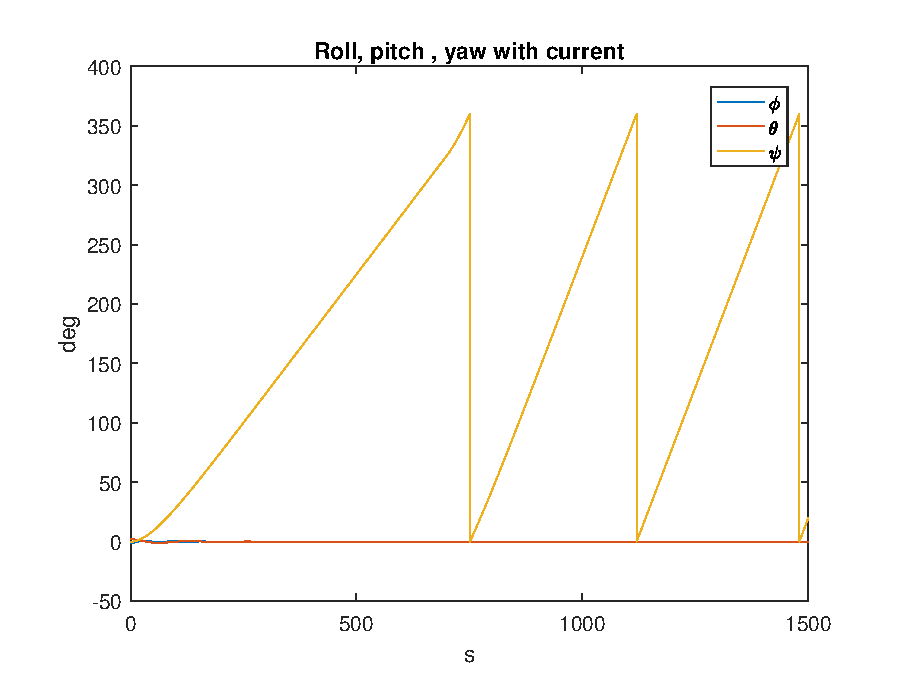
\includegraphics[width=0.6\textwidth]{figures/2_6_ang.eps}
	\caption{Plot of euler angles}
	\label{fig:2_6_ang}
\end{figure}

\begin{figure}[!ht]
	\centering
	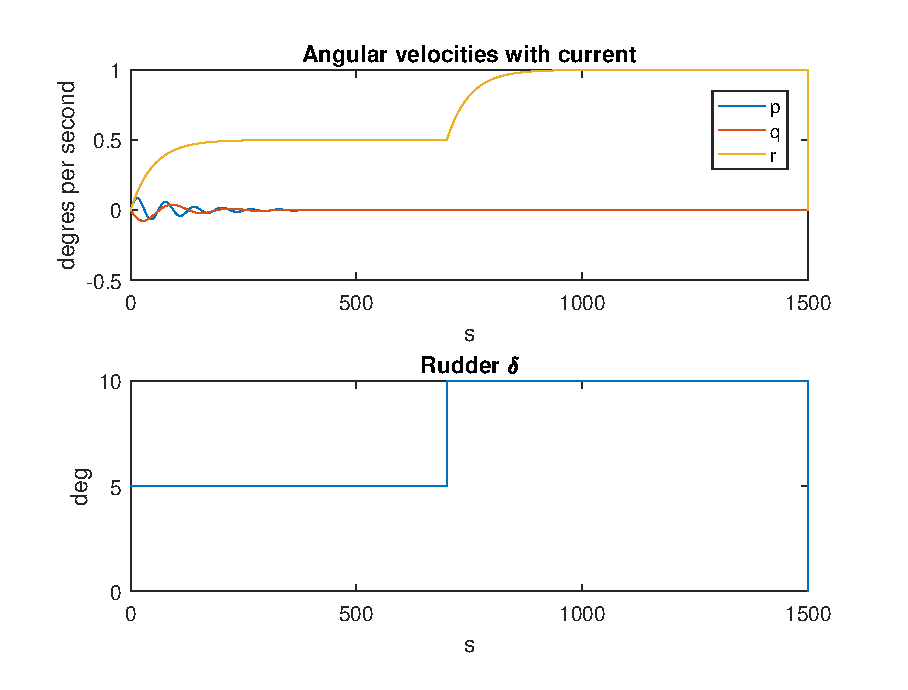
\includegraphics[width=0.6\textwidth]{figures/2_6_ang_vel.eps}
	\caption{Plot of angular velocities $\omega^b_{b/n}$}
	\label{fig:2_6_ang_vel}
\end{figure}

The plot of the position of the vehicle relative to NED in NED reference frame is represented in \ref{fig:2_6_pos}, both with and without current. In the plot with current,  \ref{fig:2_6_pos_current} the shape is similar to the plot of the vehicle moving in a circle, \ref{fig:4_pos_current}. The difference is that this time the radius of the circles changes. This is more apparent in the position plot of the vehicle without current,  \ref{fig:2_6_pos_without_current}. In this figure we see that the vehicle first approaches a larger circle as the r increases to its steady state, resulting in a decrease in the circle radius before reaching steady state and before the change in rudder is made. This is as expected from real world experience. When the rudder changes at 700 seconds, it start on a "new circle" which intersects with the old bigger circle. Looking at \ref{fig:2_6_pos_without_current} it shows that the circle increases it's radius as time increases which does not coincide with our real world experience. This happens due to a unrealistic simplification of the model of the vehicle. When the rudder suddenly increases this simultaneously affects the velocity, from \figref{fig:2_6_vel} a), affecting the frequency of the signal. The result of the sudden change in frequency of the velocity is the increasing radius of the circle. Trying different switching times, different results are achieved on the form of the new circle. A switching time better matching the changing the "form" and "frequency" of the velocity, implies better matching of the frequency.  

The reason for the first circle not having increasing radius, is because the start velocity was $\mathbf{0}$, meaning there was no mismatching of frequencies.  \todo{enig alexandra ?}

Looking back at the figure representing the relative velocity of the vehicle the same discussion above also applies when the current is not zero. First the vehicle tries to drive in a bigger circle, but because of the current, the circle becomes a spiral relative to NED. It is also apparent that it takes some time after the step at 700 seconds in rudder, before the vehicle have a relative velocity such that the "circle" has a constant radius.

\begin{figure}[!ht]
	\centering
	\begin{subfigure}[b]{0.45\textwidth}
		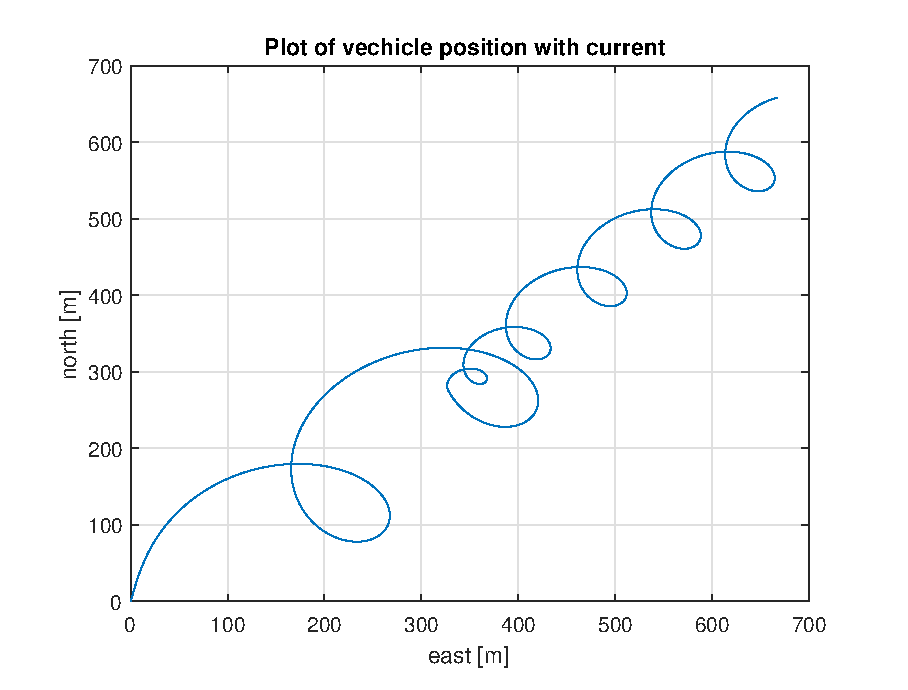
\includegraphics[width=\textwidth]{figures/2_6_pos_cur}
		\caption{Without current}
		\label{fig:2_6_pos_without_current}
	\end{subfigure}
	~ %add desired spacing between images, e. g. ~, \quad, \qquad, \hfill etc. 
	%(or a blank line to force the subfigure onto a new line)
	\begin{subfigure}[b]{0.45\textwidth}
		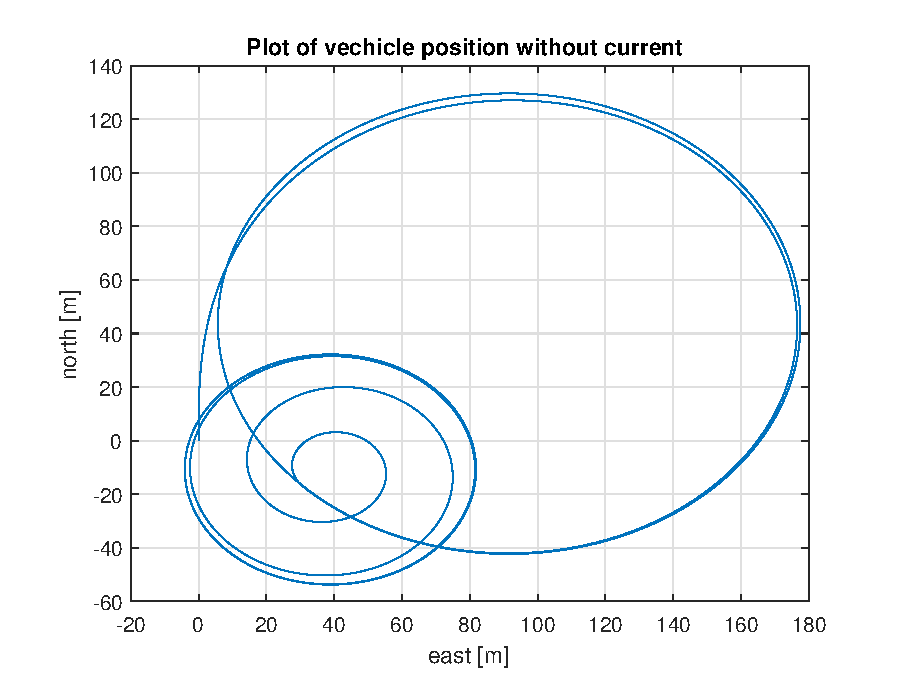
\includegraphics[width=\textwidth]{figures/2_6_pos}
		\caption{With current}
		\label{fig:2_6_pos_current}
	\end{subfigure}
	\caption{The position of the vehicle relative to NED  in reference frame NED}
	\label{fig:2_6_pos}
\end{figure}

The velocity and speed of the vehicle relative to NED and the velocity of the vehicle relative to current, both in reference frame NED is shown in figure \figref{fig:2_6_vel}. As discussed with the angular velocity $r$, this has a transient which also affects the frequency of the velocity of the vehicle. From the plot it is barley noticeable in the beginning that the periodically velocity increases the frequency of its signal. At 700 seconds, when the rudder changes, the velocities suddenly have a huge change in frequency, as discussed before. The velocity approaches a stable frequency at the same time as the rudder reaches steady state. \todo{should i discuss more about rudder ?}. Looking at the relative speed in NED vs. the relative speed to the current of the vehicle, in reference frame NED, they have similar form, but the velocity relative to NED have elevated zero compared to the velocity relative to the current, which is consistent with constant current. This is the same result as before. The speed behaves as before, with constant speed relative to current, and changing speed relative to NED. The speed relative to NED is also, of course, due to the sudden change in frequency.

\begin{figure}[!ht]
	\centering
	\begin{subfigure}[b]{0.45\textwidth}
		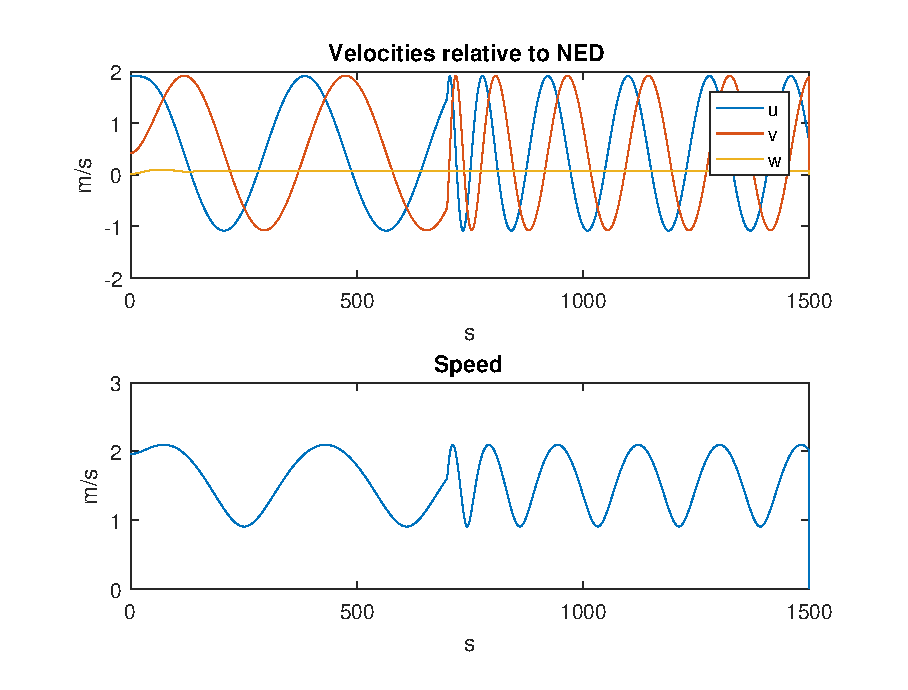
\includegraphics[width=\textwidth]{figures/2_6_vel_ned}
		\caption{Without current}
		%\label{fig:4_vel}
	\end{subfigure}
	~ %add desired spacing between images, e. g. ~, \quad, \qquad, \hfill etc. 
	%(or a blank line to force the subfigure onto a new line)
	\begin{subfigure}[b]{0.45\textwidth}
		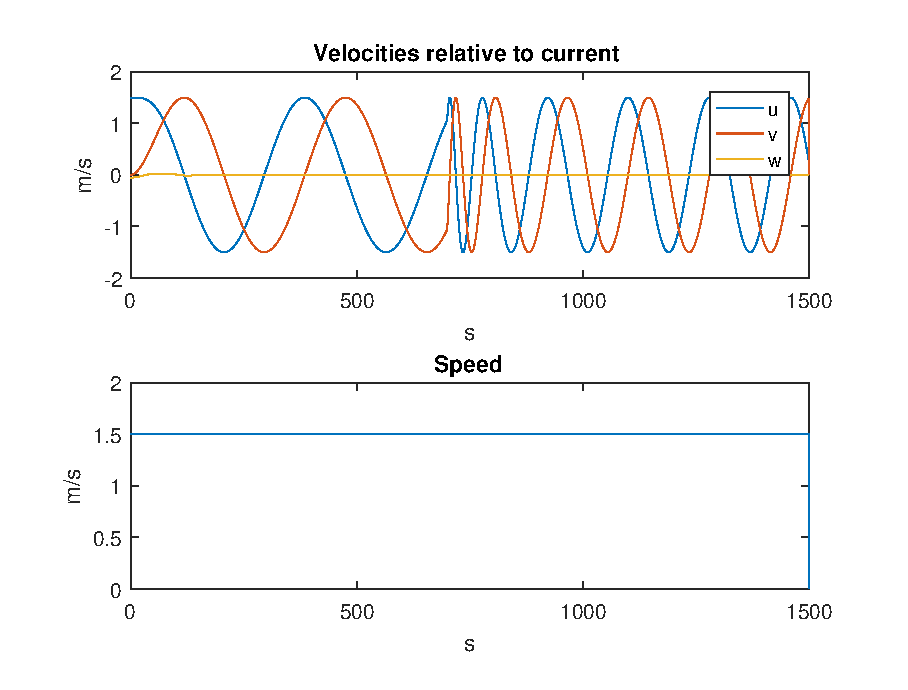
\includegraphics[width=\textwidth]{figures/2_6_vel_cur}
		\caption{With current}
		%\label{fig:4_vel_ned_with_cur}
	\end{subfigure}
	\caption{The velocity of the vehicle relative to NED  in reference frame NED}
	\label{fig:2_6_vel}
\end{figure}

The graphs of the crab angle, sideslip angle and course angle are plotted in figure \figref{fig:2_6_crab}. The figure shows that the sideslip angle increases linearly, as in problem 2.5 because it is only depending on $\mathbf{v}^b_{b/c}$. The only change in sideslip is when the frequency of the relative velocity changes, according to the change in rudder. After the change in rudder the sideslip angle have an increase in frequency (rate of going from $0 - 360 ^\circ$), which is as expected the the vehicle runs on a small circle, with same relative velocity.

As previously discussed the crab angle and the course angle depends on $\mathbf{v}^b_{b/n}$, meaning that the angle does not have linear slope. Because of the rotation of the vehicle, the yaw is not constant, as in the previous assignments. This affects the course angle so as to have to have a shorter period, going from $0-360^\circ$. The crab angle is only affected by $\mathbf{v}^n_{b/c}$ meaning it has almost the same shape as in problem 2.4 when the angular velocity $r$ is in steady state. When the $r$ is not steady state the crab angle behaves differently. The transient in the angular velocity $r$ is mostly noticeable at 700 seconds. This is because of the sudden change in rudder and mismatch of frequencies in the velocities, as discussed before. After 700 seconds, all the angles in \figref{fig:2_6_crab} have faster frequencies than before 700 s,changing from 0-360 degrees because of faster frequency in the velocity.  \todo{makes it sense to talk about frequency to angle ? }.

\begin{figure}[!ht]
	\centering
	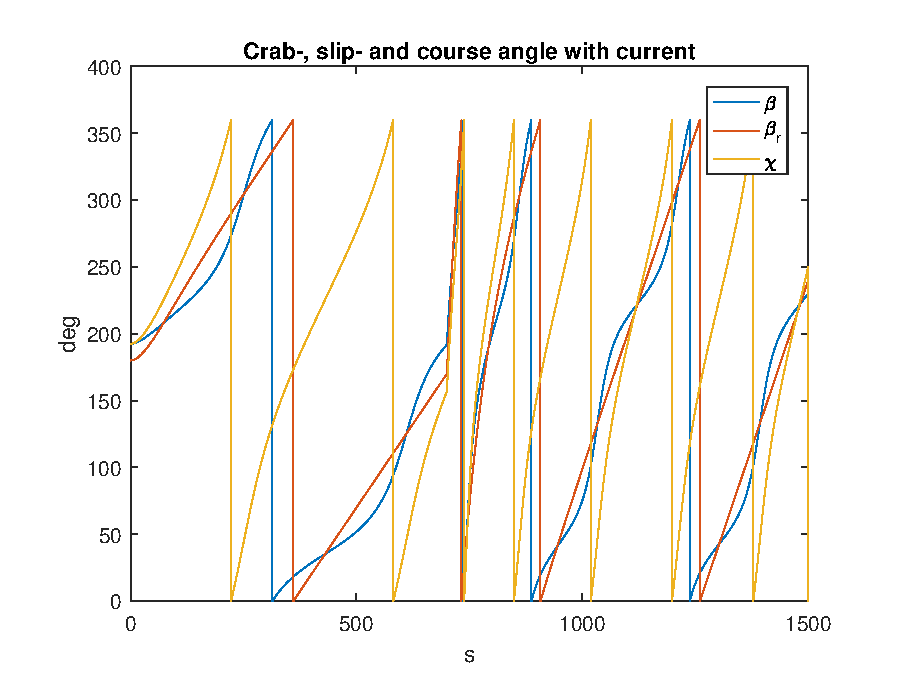
\includegraphics[width=0.6\textwidth]{figures/2_6_crab_slip_course.eps}
	\caption{Plot of the crab-, slip- and course angle}
	\label{fig:2_6_crab}
\end{figure}
% laplace reference : http://tutorial.math.lamar.edu/pdf/Laplace_Table.pdf
%\section*{Problem 2 - Underwater Vehicles}
Answer Problem 2 in this file. 
\subsection*{Problem 2.1}
Answer problem 2.1 here. The Greek letters for sideslip, crab and course are $\beta_r$, $\beta$ and $\chi$, respectively. The Greek letter for the flight-path angle is $\gamma$.

\subsection*{Problem 2.2}
Answer Problem 2.2 here. The body-fixed velocities can be written as
\begin{equation}
\label{eq:velocity}
	\begin{bmatrix}
		u \\
		v \\
		w
	\end{bmatrix}
	= 
	\begin{bmatrix}
		U \cos( \omega t)\\
		U \sin(\omega t)\\
		0	
	\end{bmatrix}
\end{equation}

\subsection*{Problem 2.3}
Answer Problem 2.3 here.

\subsection*{Problem 2.4}
Answer Problem 2.4 here. Figures can be inserted as:
\begin{figure}[ht]
	\centering
	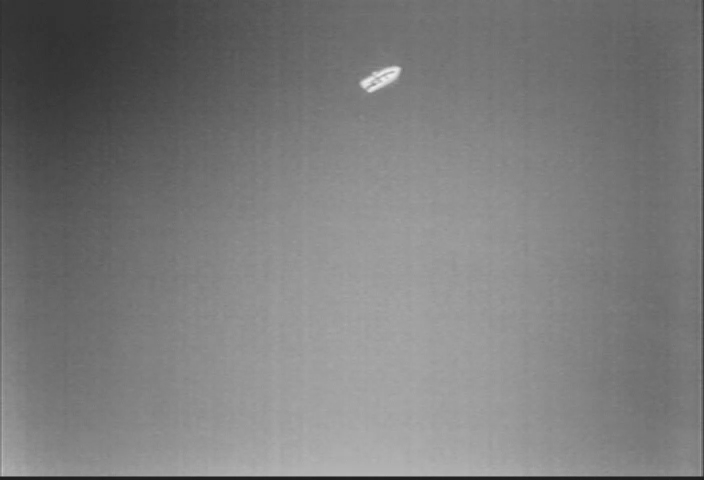
\includegraphics[width=0.7\textwidth]{fig1} % Filename is "fig1.png" and must be located in the same folder as this file. If you have a folder containing all the figures you can use "Figures/fig 1" as long as the "Figures" folder is placed in the same folder as this file.
	\caption{Figure of something useful.}
	\label{fig:fig1}
\end{figure}

You can now refer to this figure as \figref{fig:fig1}. You can also insert figures side-by-side:
\begin{figure}[ht]
	\centering
	\begin{subfigure}[b]{0.45\textwidth}
		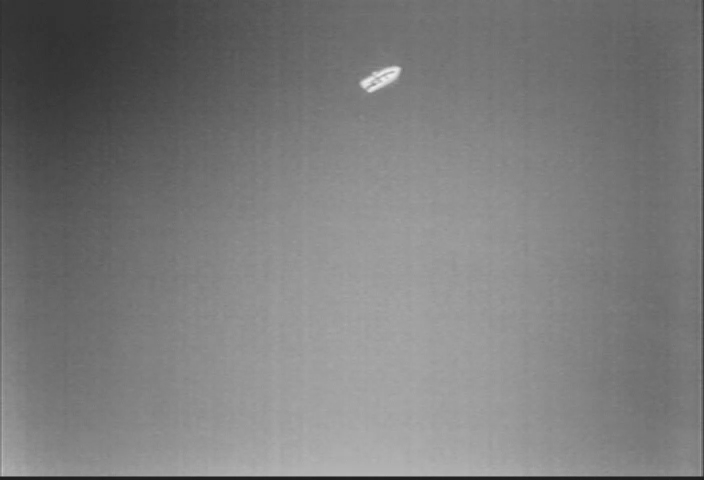
\includegraphics[width=\textwidth]{fig1}
		\caption{caption..}
		\label{fig:2a}
	\end{subfigure}
	~ %add desired spacing between images, e. g. ~, \quad, \qquad, \hfill etc. 
	%(or a blank line to force the subfigure onto a new line)
	\begin{subfigure}[b]{0.45\textwidth}
		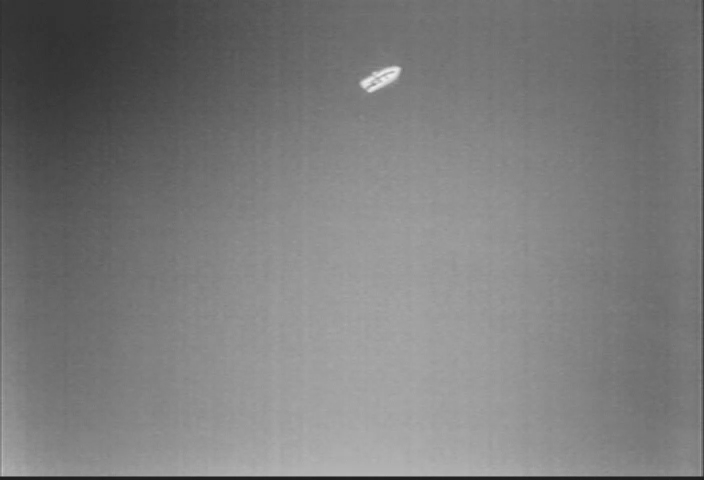
\includegraphics[width=\textwidth]{fig1}
		\caption{caption..}
		\label{fig:2b}
	\end{subfigure}
	\begin{subfigure}[b]{0.45\textwidth}
		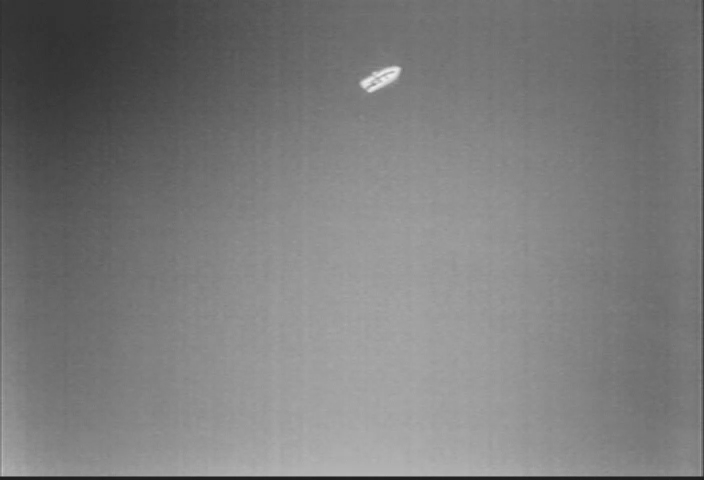
\includegraphics[width=\textwidth]{fig1}
		\caption{caption..}
		\label{fig:2c}
	\end{subfigure}
	\begin{subfigure}[b]{0.45\textwidth}
		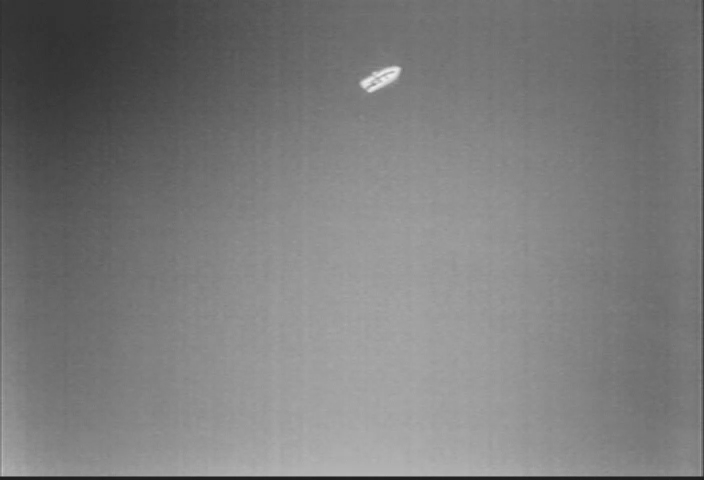
\includegraphics[width=\textwidth]{fig1}
		\caption{caption..}
		\label{fig:2d}
	\end{subfigure}		
	\caption{Caption for all figures}\label{fig:2}
\end{figure}

\subsection*{Problem 2.5}
The Nomoto model can be written as
\begin{equation}
	\frac{r}{\delta} (s) = \frac{K}{Ts+1}
\end{equation}
and the equations for the roll and pitch rate as
\begin{equation}
\begin{aligned}
	&\dot{p} + 2\zeta_p\omega_p p + \omega_p^2 \phi = 0\\
	&\dot{q} + 2\zeta_q\omega_q q + \omega_q^2 \theta = 0
\end{aligned}
\end{equation}

\subsection*{Problem 2.6}
References can be placed in the bibliography.bib and referred to as \cite{Fossen2011} and \cite{Fjellstad1994857}.

%\section{Conclusion}\label{sec:conclusion}

In this project, optimal control with and without feedback was implemented on the following in-flight measures of the helicopter under control:
\begin{itemize}
    \item  Pitch/Travel 
    \item  Pitch/Travel and Elevation 
\end{itemize}

The results from this optimization in both cases strongly suggest that the helicopter is controlled better with feedback than without, according to the goal of travelling from $\lambda = \pi $ to $\lambda = 0$. The feedback-less control would have fared somewhat better with a more elaborate and accurate model, ideally taking into account noise as well. The model based errors were somewhat counteracted through feedback, as well as noise such as random winds from surrounding airspace.
The model error because of the dependencies between the angles were one of the most dominant errors, such that it was difficult to have both pitch and travel the optimal planned path.  

During this project we gained practice in formulating a dynamic optimization problem, as well as discretizing and solving the resulting problem using a computer. We gained experience with the implementation and practical use of optimal control with and without feedback.



%\addcontentsline{toc}{section}{Appendix} \label{sec:appendix}
\appendix

\section{MATLAB Code}\label{sec:matlab}

Section contains \texttt{MATLAB}-code this project. Code posted online on BlackBoard are not in the Appendix. 

\subsection{Calculating discrete model, observability matrix and controllability matrix for 4 states} \label{sec:disk_2}
%\lstinputlisting{code/plot_constraint.m}

\begin{lstlisting}[
    language=Matlab,escapechar=|, label={lst:disk_2}, caption={Calculating discrete model for problem 2}]
    %% Model for Ex. 4

    A_c = [ 0 1 0 0 0 0; 
            0 0 -K_2 0 0 0; 
            0 0 0 1 0 0; 
            0 0 -K_1*K_pp -K_1*K_pd 0 0;
            0 0 0 0 0 1; 
            0 0 0 0 -K_3*K_ep -K_3*K_ed ];
    B_c = [ 0 0; 
            0 0; 
            0 0; 
            K_1*K_pp 0;
            0 0; 
            0 K_3*K_ed];
    
    
    %% Forward Euler method
    deltaT = 0.25;
    I = diag([1,1,1,1,1,1]);
    
    A_d = (I + deltaT*A_c);
    B_d = deltaT * B_c;
    
    %% Stabilizible:

    C= ctrb(A_d,B_d)
    rank(C)
    %% Detectable
    
    O = obsv(A_d,C_d)
    rank(O)
    
    %% LQR
    Q = diag([10 2 1 2]);
    R = 1;
    K = dlqr(A_d,B_d,Q,R);   
\end{lstlisting}

\subsection{Calculation of the optimal input sequence with 4 states }

\begin{lstlisting}[
    language=Matlab,escapechar=|, label={lst:main_code_2}, caption={Calculation of the optimal input sequence with 4 states }] 
    
    % TTK4135 - Helicopter lab
    % The code is heavily based on 
    % the hints/template for problem 2.
    % Updated spring 2017, Andreas L. Fl?ten
    
    %% Initialization and model definition
    init; % Init file for our helicopter
    Discrete_model_euler;
    delta_t	= 0.25; % sampling time
    
    % Discrete time system model. x = [lambda r p p_dot]'
    A1 = A_d % From the discrete computation
    B1 = B_d 
    
    % Number of states and inputs
    mx = size(A1,2); % Number of states (number of columns in A)
    mu = size(B1,2); % Number of inputs(number of columns in B)
    
    % Initial values
    x1_0 = pi;                              % Lambda
    x2_0 = 0;                               % r
    x3_0 = 0;                               % p
    x4_0 = 0;                               % p_dot
    x0 = [x1_0 x2_0 x3_0 x4_0]';          % Initial values
    
    % Time horizon and initialization
    N  = 100;                                % Time horizon for states
    M  = N;                                 % Time horizon for inputs
    z  = zeros(N*mx+M*mu,1);                % Initialize z for the whole horizon
    z0 = z;                                 % Initial value for optimization
    
    % Bounds
    ul 	    = -30*pi/180;                   % Lower bound on control - u1
    uu 	    = 30*pi/180;                    % Upper bound on control - u1
    
    xl      = -Inf*ones(mx,1);              % Lower bound on states (no bound)
    xu      = Inf*ones(mx,1);               % Upper bound on states (no bound)
    xl(3)   = ul;                           % Lower bound on state x3
    xu(3)   = uu;                           % Upper bound on state x3
    
    % Generate constraints on measurements and inputs
    [vlb,vub]       = genbegr2(N,M,xl,xu,ul,uu); 
    vlb(N*mx+M*mu)  = 0;                    % We want the last input to be zero
    vub(N*mx+M*mu)  = 0;                    % We want the last input to be zero
    
    % Generate the matrix Q and the vector c (objecitve function weights in the QP problem) 
    Q1 = zeros(mx,mx);
    Q1(1,1) = 1;                             % Weight on state x1
    Q1(2,2) = 0;                            % Weight on state x2
    Q1(3,3) = 0;                             % Weight on state x3 
    Q1(4,4) = 0;                            % Weight on state x4 
    P1 = 1;                                 % Weight on input
    Q = 2*genq2(Q1,P1,N,M,mu);              % Generate Q
    c = zeros(N*mx+M*mu,1);                 % Generate c
    
    %% Generate system matrixes for linear model
    Aeq = gena2(A1,B1,N,mx,mu);           % Generate A
    beq = zeros(M*mx, 1);        	  % Generate b
    beq(1:mx) = A1*x0; % Initial value
    
    %% Solve QP problem with linear model
    tic
    [z,lambda] = quadprog(Q, c, [], [], Aeq, beq, vlb, vub); 
    t1=toc;
    
    % Calculate objective value
    phi1 = 0.0;
    PhiOut = zeros(N*mx+M*mu,1);
    for i=1:N*mx+M*mu
      phi1=phi1+Q(i,i)*z(i)*z(i);
      PhiOut(i) = phi1;
    end
    
    %% Extract control inputs and states
    u  = [z(N*mx+1:N*mx+M*mu);z(N*mx+M*mu)]; |\label{line:extract_vals}| % Control input from solution 
    
    x1 = [x0(1);z(1:mx:N*mx)];              % State x1 from solution
    x2 = [x0(2);z(2:mx:N*mx)];              % State x2 from solution
    x3 = [x0(3);z(3:mx:N*mx)];              % State x3 from solution
    x4 = [x0(4);z(4:mx:N*mx)];              % State x4 from solution
    
    num_variables = 5/delta_t;|\label{line:zero_padding_start}|
    zero_padding = zeros(num_variables,1);
    unit_padding  = ones(num_variables,1);
    
    u   = [zero_padding; u; zero_padding]; 
    x1  = [pi*unit_padding; x1; zero_padding];
    x2  = [zero_padding; x2; zero_padding];
    x3  = [zero_padding; x3; zero_padding];
    x4  = [zero_padding; x4; zero_padding];|\label{line:zero_padding_end}|
    
    %% Plotting
    t = 0:delta_t:delta_t*(length(u)-1); |\label{line:plotting2}|
    input = [t' u]; 
    figure(2)
    hold on;
    subplot(511)
    stairs(t,u),grid
    ylabel('u')
    subplot(512)
    plot(t,x1,'m',t,x1,'mo'),grid
    ylabel('lambda')
    subplot(513)
    plot(t,x2,'m',t,x2','mo'),grid
    ylabel('r')
    subplot(514)
    plot(t,x3,'m',t,x3,'mo'),grid
    ylabel('p')
    subplot(515)
    plot(t,x4,'m',t,x4','mo'),grid
    xlabel('tid (s)'),ylabel('pdot')
\end{lstlisting}

\newpage


\subsection{Calculating controllability, observability matrix and LQR for 6 states }\label{sec:matlab_4_2}

\begin{lstlisting}[
    language=Matlab,escapechar=|, caption={Calculating controllability matrix, observability matrix and LQR for 6 states}, label={lst:matlab_4_2}]

%% Model for Ex. 4
A_c = [0 1 0 0 0 0;
       0 0 -K_2 0 0 0;
       0 0 0 1 0 0;
       0 0 -K_1*K_pp -K_1*K_pd 0 0; 
       0 0 0 0 0 1;
       0 0 0 0 -K_3*K_ep -K_3*K_ed ];
       
B_c = [0 0;
       0 0;
       0 0;
       K_1*K_pp 0;
       0 0;
       0 K_3*K_ed];

%% Forward Euler method
deltaT = 0.25;
I = diag([1,1,1,1,1,1]);

A_d = (I + deltaT*A_c);
B_d = deltaT * B_c;

%% Stabilizable
C = ctrb(A_d,B_d);
rank(C)

%% Detectable
O = obsv(A_d,C_d)
rank(O)

%% Calculate K
Q = diag([20 1 100 2 300000 500]);
R = [1 0; 0 1];
K = dlqr(A_d,B_d,Q,R);   
    
\end{lstlisting}
\newpage

\subsection{Non-linear constraint on elevation }\label{sec:matlab_connstrains}
\begin{lstlisting}[
    language=Matlab,escapechar=|, caption={Non-linear constraint on elevation}]

function [ c, ceq ] = nonlinearconstraints(z)
    
    global N;
    global mx;
    size(N);
    size(mx);
    
    alpha = 0.2;
    beta = 20;
    lambda_t = 2*pi/3;
    c = zeros(N,1);
    for i = 0:(N-1)
        c(i+1) = alpha*exp(-beta*(z(1 +mx*i) - lambda_t)^2) - z(5 +mx*i);
    end

    ceq = [];
    
\end{lstlisting}

\subsection{Calculation of the optimal input sequence with 6 states }\label{sec:matlab_4_3}

\begin{lstlisting} [
    language=Matlab,escapechar=|, label={lst:main_code_4}, caption={Calculation of the optimal input sequence with 6 states}]

% TTK4135 - Helicopter lab
% Hints/template for problem 2.
% Updated spring 2017, Andreas L. Fl?ten

%% Initialization and model definition
init; 
Discrete_model_euler;
delta_t	= 0.25; % sampling time
global N;
global mx;
global M;

% Discrete time system model. 
A1 = A_d; 
B1 = B_d; 

% Number of states and inputs
mx = size(A1,2); % Number of states 
mu = size(B1,2); % Number of inputs

% Initial values
x0 = [ pi 0 0 0 0 0 ]';          

% Time horizon and initialization
N  = 40;            % Time horizon for states
M  = N;             % Time horizon for inputs
z  = zeros(N*mx+M*mu,1);                    
z0 =z; 

% Bounds
pitch_lim = 30*pi/180; |\label{line:start_limit}|
pitch_rate_lim = inf; %20*pi/180;
elevation_lim = inf;
ul =[-pitch_lim; -elevation_lim];
uu =[pitch_lim; elevation_lim];

xl      = [-inf -inf -pitch_lim -pitch_rate_lim -inf -inf]';              % Lower bound on states 
xu      = [inf inf pitch_lim pitch_rate_lim inf inf]';               % Upper bound on states 

% Generate constraints on measurements and inputs
[vlb,vub]       = genbegr2(N,M,xl,xu,ul,uu);|\label{line:end_limit}| ;

% Generate the matrix Q and R and G (objecitve function weights in the QP problem) 
Q1 = diag([1 0 0 0 0 0]);
R = diag([1 1]);
G = 2*genq2(Q1,R,N,M,mu); |\label{line:4_G}|

%% Generate system matrixes for linear model
Aeq = gena2(A1,B1,N,mx,mu) |\label{line:start_eq}|; beq = zeros(M*mx, 1);        
beq(1:mx) = A1*x0 |\label{line:end_eq}|; % Initial value

%% Objective function
f = @(Z) Z'*G*Z;

%% SQP
options = optimoptions('fmincon','Algorithm','sqp','MaxFunEvals',60000);
tic
Z = fmincon(f, z0, [], [], Aeq, beq, vlb, vub, @nonlinearconstraints, options); |\label{line:4_fmincon}|
t1=toc;

%% Extract control inputs and states
u1  = [Z(N*mx+1:mu:N*mx+M*mu); Z(N*mx + M*mu - 1)]; 
u2 = [Z(N*mx+2:mu:N*mx+M*mu); Z(N*mx + M*mu)];


x1 = [x0(1);Z(1:mx:N*mx)];              
x2 = [x0(2);Z(2:mx:N*mx)];              
x3 = [x0(3);Z(3:mx:N*mx)];              
x4 = [x0(4);Z(4:mx:N*mx)];              
x5 = [x0(5);Z(5:mx:N*mx)];              
x6 = [x0(6);Z(6:mx:N*mx)];              

num_variables = 5/delta_t;
zero_padding = zeros(num_variables,1);
unit_padding  = ones(num_variables,1);

u1   = [zero_padding; u1; zero_padding];
u2   = [zero_padding; u2; zero_padding];
u = [u1 u2];
x1  = [pi*unit_padding; x1; zero_padding];
x2  = [zero_padding; x2; zero_padding];
x3  = [zero_padding; x3; zero_padding];
x4  = [zero_padding; x4; zero_padding];
x5  = [zero_padding; x5; zero_padding];
x6  = [zero_padding; x6; zero_padding];
x = [x1 x2 x3 x4 x5 x6];

%% LQR
Q = diag([20 1 100 2 300000 500]);
R = [1 0; 0 1];
K = dlqr(A1,B1,Q,R);      
% 
%% Plotting
t = 0:delta_t:delta_t*(length(u)-1);
input_opt = [t' u]; 
x_opt = [t' x];

\end{lstlisting}



\section{Simulink Diagrams}

\subsection{Diagram from implementation of optimal control of pitch/travel without feedback}

\begin{figure}[!h]
    \centering
	\includegraphics[width=1.2\textwidth]{figures/part2/simulink_lab2.PNG}
	\caption{Simulink diagram for Optimal Control of Pitch/Travel without Feedback}
\label{fig:L2_sim}
\end{figure}

\newpage

\subsection{Diagrams from implementation of optimal control of pitch/travel with feedback}\label{sec:simmulink_3_2}

\begin{figure}[!h]
	\centering
	\includegraphics[width=1.00\textwidth]{figures/part3/im_3_2_full.PNG}
	\caption{Simulink diagram of the system implemented with feedback and LQR-controller.}
    \label{fig:3_2_full}
\end{figure} 

\begin{figure}[!h]
	\centering
	\includegraphics[width=1.00\textwidth]{figures/part3/im_3_2_u.PNG}
	\caption{Feedback implemented in system}
    \label{fig:3_2_u}
\end{figure} 


\newpage

\subsection{Diagram from implementation of optimal control of pitch/travel and elevation with
and without feedback}

\begin{figure}[!h]
    \centering
	\includegraphics[width=1.2\textwidth]{figures/part4/sim_4_open_loop.PNG}
	\caption{Simulink diagram for Optimal Control of Pitch/Travel and Elevation without Feedback}
\label{fig:L4_sim_open}
\end{figure}

\begin{figure}[!h]
    \centering
	\includegraphics[width=1.2\textwidth]{figures/part4/sim_4_closed_loop.PNG}
	\caption{Simulink diagram for Optimal Control of Pitch/Travel and Elevation with Feedback}
\label{fig:L4_sim_closed}
\end{figure}

\begin{figure}[!h]
    \centering
	\includegraphics[width=1.2\textwidth]{figures/part4/sim_4_closed_loop_inside_control.PNG}
	\caption{Inner simulink diagram of the 'Optimal Control' box from \Cref{fig:L4_sim_closed}}
\label{fig:L4_sim_closed_control}
\end{figure}

\newpage

\newpage
\addcontentsline{toc}{section}{References}
\printbibliography
\label{sec:bibliography}


\end{document}
